% !TEX root = ./notes_template.tex
%%%%%%%%%%%%%%%%%%%%%%%%%%%%%%%%%%%%%%%%%%%%%%%%%%
%%%%%%%%%%%%%%%%%%%%% preamble %%%%%%%%%%%%%%%%%%%
%%%%%%%%%%%%%%%%%%%%%%%%%%%%%%%%%%%%%%%%%%%%%%%%%%
\documentclass[12pt]{report}
%\documentclass[11pt,twoside]{book}
\renewcommand{\chaptername}{Week}
% Font and layout
\usepackage[mono=false]{libertine} % Font family
%\usepackage{geometry}
%\geometry{margin=2.5cm}
\usepackage[left=2.5cm, right=2.5cm, top=2cm, bottom=2cm]{geometry}

% Math and symbols
\usepackage{amsmath,amssymb}
\usepackage{bm}
\usepackage{amssymb}

% Figures and graphics
\usepackage{graphicx}
\usepackage{subcaption}
\usepackage{caption}
\usepackage{float}

% Tables
\usepackage{tabularx}
\usepackage{multirow}

% Lists and formatting
\usepackage{enumitem}

% Hyperlinks and references
\usepackage{hyperref}
\hypersetup{
    colorlinks=true,
    citecolor=magenta,
    linkcolor=blue,
    filecolor=green,
    urlcolor=cyan
}
\usepackage[capitalise]{cleveref}

% Custom boxes for lab activities
\usepackage{tcolorbox}
\newtcolorbox{labactivitybox}{
  colback=gray!10,
  colframe=black,
  fonttitle=\bfseries,
  title=Lab Activity,
  left=1em,
  right=1em,
  top=1em,
  bottom=1em,
  boxrule=0.5pt,
  arc=4pt
}



%%%%%%%%%%%%%%%% ToC %%%%%%%%%%%%%%%%%%%%%
% Link Chapter title to ToC: https://tex.stackexchange.com/questions/32495/linking-the-section-text-to-the-toc
\usepackage[explicit]{titlesec}
\titleformat{\chapter}[display]
  {\normalfont\huge\bfseries}{\chaptertitlename\ {\thechapter}}{20pt}{\hyperlink{chap-\thechapter}{\Huge#1}
\addtocontents{toc}{\protect\hypertarget{chap-\thechapter}{}}}
\titleformat{name=\chapter,numberless}
  {\normalfont\huge\bfseries}{}{-20pt}{\Huge#1}

%%%%%%%%%%%%%%%%%%% fancyhdr - Customized for Lab Manual %%%%%%%%%%%%%%%%%
\usepackage{fancyhdr}
\pagestyle{fancy}
\renewcommand{\headrulewidth}{0.0pt} % remove header rule
\fancyhf{} % clear header and footer

% Define header layout
\fancyhead[LO,LE]{\nouppercase{\leftmark}} % Week title
\fancyhead[RO,RE]{\textbf{Week \thechapter}} % Week number
\fancyfoot[CE,CO]{\hyperref[toc-contents]{\thepage}} % clickable page number

% Update chapter and section marks with "Week" and link support
\makeatletter
\renewcommand{\chaptermark}[1]{%
  \markboth{\protect\hyper@linkstart{link}{\@currentHref}{Week \thechapter\quad #1}\protect\hyper@linkend}{}}
\renewcommand{\sectionmark}[1]{%
  \markright{\protect\hyper@linkstart{link}{\@currentHref}{\thesection\quad #1}\protect\hyper@linkend}}
\makeatother
%%%%%%%%%%%%%%%%%%% fancyhdr %%%%%%%%%%%%%%%%%


%%%%%%%%%%%%%%%%%%% biblatex %%%%%%%%%%%%%%%%%
\usepackage[doi=false,url=false,isbn=false,style=alphabetic,backend=biber,backref=true]{biblatex}
\addbibresource{bib.bib}

\newbibmacro{string+doiurlisbn}[1]{%
  \iffieldundef{doi}{%
    \iffieldundef{url}{%
      \iffieldundef{isbn}{%
        \iffieldundef{issn}{%
          #1%
        }{%
          \href{http://books.google.com/books?vid=ISSN\thefield{issn}}{#1}%
        }%
      }{%
        \href{http://books.google.com/books?vid=ISBN\thefield{isbn}}{#1}%
      }%
    }{%
      \href{\thefield{url}}{#1}%
    }%
  }{%
    \href{http://dx.doi.org/\thefield{doi}}{#1}%
  }%
}

% https://tex.stackexchange.com/questions/94089/remove-quotes-from-inbook-reference-title-with-biblatex
\DeclareFieldFormat[article,incollection,inproceedings,book,misc]{title}{\usebibmacro{string+doiurlisbn}{\mkbibemph{#1}}}
% https://tex.stackexchange.com/questions/454672/biblatex-journal-name-non-italic
\DeclareFieldFormat{journaltitle}{#1\isdot}
\DeclareFieldFormat{booktitle}{#1\isdot}
% https://tex.stackexchange.com/questions/10682/suppress-in-biblatex
\renewbibmacro{in:}{}
% add video field: https://tex.stackexchange.com/questions/111846/biblatex-2-custom-fields-only-one-is-working
\DeclareSourcemap{
    \maps[datatype=bibtex]{
      \map{
        \step[fieldsource=video]
        \step[fieldset=usera,origfieldval]
    }
  }
}
\DeclareFieldFormat{usera}{\href{#1}{\textsc{Online video}}}
\AtEveryBibitem{
    \csappto{blx@bbx@\thefield{entrytype}}{% put at end of entry
        \iffieldundef{usera}{}{\space \printfield{usera}}
    }
}
%%%%%%%%%%%%%%%%%%% biblatex %%%%%%%%%%%%%%%%%


\input{./macros.tex}

%%%%%%%%%%%%%%%%%%%%%%%%%%%%%%%%%%%%%%%%%%%%%%%%%%
%%%%%%%%%%%%%%%% begin of document %%%%%%%%%%%%%%%
%%%%%%%%%%%%%%%%%%%%%%%%%%%%%%%%%%%%%%%%%%%%%%%%%%

\begin{document}

\title{{\Large A Lab Manual for the:}\\
[0.5em]{\bf \Huge Neuromuscular \& Vascular Lab}\\
[0.5em]{\Large Functional Movement, Manual Testing \& Rehabilitative Ultrasound Imaging}}

\author{Sean Collins, Janine DeBaets \& Kaylee Pobocik \\
{\small Instructional support assisted by the Clinical Anatomy Lab Assistant GPT (OpenAI),}\\
{\small a custom tool designed by Sean Collins for the Plymouth State DPT Program.}}





\date{Update on \today}
\maketitle
\thispagestyle{empty}
\vspace*{3cm}

\begin{center}
\textbf{Neuromuscular \& Vascular Lab Manual} \\
\textit{Functional Movement, Manual Testing \& Rehabilitative Ultrasound Imaging} \\[1em]

Sean Collins, Janine DeBaets \& Kaylee Pobocik \\
Instructional development supported by the Clinical Anatomy Lab Assistant GPT (OpenAI) \\[3em]

\textcopyright{} 2025 Sean Collins, Janine DeBaets \& Kaylee Pobocik \\
Published by PT Centered Press, Ashland, NH 03217 \\[1em]

\textbf{All rights reserved.}

No part of this publication may be reproduced, stored in a retrieval system, or transmitted in any form or by any means—electronic, mechanical, photocopying, recording, or otherwise—without the prior written permission of the author or publisher. \\[2em]

This manual is intended for instructional use within the Plymouth State University Doctor of Physical Therapy Program. \\
For permissions or inquiries, contact: \texttt{smcollins1@plymouth.edu}
\end{center}

\vspace{2em}
\noindent\textit{Note to the reader:} This is the first full implementation of the \textit{Neuromuscular \& Vascular Lab Manual} in its integrated format: combining manual muscle tests, muscle length tests, deep tendon reflexes, vascular palpation and rehabilitative ultrasound imaging. While each element has been taught previously, this is the first time they are scaffolded together throughout the lab curriculum. Your experience and feedback are essential for refining the manual for future cohorts.

\vfill 
\setcounter{tocdepth}{2}
\tableofcontents
%%%%%%%%%%%%%%%Content%%%%%%%%%%%%%%%

% !TEX root = ../notes_template.tex
\chapter*{Preface}
\addcontentsline{toc}{chapter}{Preface}

The \textit{Neuromuscular \& Vascular Lab} is a foundational component of your first semester in the Plymouth State University Doctor of Physical Therapy Program. While embedded in \textbf{PTH6110 Clinical \& Functional Anatomy}, this lab serves as the anatomical counterpart to \textbf{PTH6111 Clinical Physiology: A Muscle Centered Approach}. Together, these two courses provide a uniquely integrated experience—merging structure, function, and clinical application from the very beginning of your professional training.

This manual is your lab companion, designed to help you not only locate structures but understand how they behave, interact, and adapt in clinical contexts. Just as \textit{Clinical Physiology} centers on the muscle fiber as the generative engine of movement, this lab allows you to palpate, assess, and visualize that generation in action. When you test a muscle’s performance through manual testing, evaluate segmental contributions via reflexes and pulses, or visualize tissue with rehabilitative ultrasound imaging (RUSI), you are putting physiological principles into practice.

The lab and physiology course reinforce a shared set of core principles:
\begin{itemize}
    \item \textbf{Tension} is central to both courses: generated by muscle fibers, regulated by motor units, supported by vascular and respiratory systems.
    \item \textbf{Excitation and regulation}, key themes in physiology, come alive as you trace neurologic pathways from spinal roots to peripheral nerves to muscles during manual muscle testing.
    \item \textbf{Circulation and microcirculation}, which support extracellular fluid homeostasis in physiology, are examined in the lab through pulse assessment and RUSI.
    \item \textbf{Systems thinking}, emphasized in both, is not optional but essential: movement and dysfunction must be understood through multiregional and multisystem interactions.
\end{itemize}

This lab doesn’t just teach you where things are—it challenges you to think like a clinician. You'll begin to reason through the “why” behind what you see, feel, and test. As you explore the shoulder, pelvis, or cervical spine, remember that no movement occurs in isolation. Clinical reasoning requires that you understand both the anatomy and the physiology of functional—and dysfunctional movement—as a dynamic whole.

Use this manual actively. Annotate it. Use it to generate hypotheses. Bring insights from physiology into the lab and bring questions from the lab into your physiology discussions. When you understand how a muscle creates and sustains tension—and what can compromise that process—you are beginning to think like a physical therapist.

\vspace{2em}
\noindent\textit{Sean Collins}\\
\textit{May 2025}

% !TEX root = ../notes_template.tex
\chapter*{Tentative Schedule}
\addcontentsline{toc}{chapter}{Schedule}

\begin{center}
\begin{tabular}{|c|c|p{8cm}|}
\hline
\textbf{Date} & \textbf{Week} & \textbf{Topic} \\
\hline
June 2 & Week 1 & Movement \& Muscle Testing \\
\hline
June 9 & Week 2 & Intro to Reflexes, Pulses \& RUSI \\
\hline
June 16 & Week 3 & Shoulder Complex \\
\hline
June 23 & Week 4 & Elbow, Forearm, Wrist \& Hand \\
\hline
June 30 & Week 5 & Pelvis \& Hip \\
\hline
July 7 & Week 6 & Knee \\
\hline
July 14 & Week 7 & Ankle \& Foot \\
\hline
July 21 & Week 8 & Lumbopelvic \\
\hline
July 28 & Week 9 & Cervical \& Quarter Screens \\
\hline
Aug 4 & Week 10 & Clinical Skills Checklist \\
\hline
\end{tabular}
\end{center}

\bigskip
\noindent
\textit{Note:} Despite the regional organization of the laboratory, which is progressing anatomically from the shoulder complex to the cervical spine, its foundation of clinical reasoning remains grounded in a regional interdependence framework. The regional structure ensures that the lab content aligns directly with the concurrent lecture material and the Osteology \& Arthrology Lab, supporting consistency throughout the summer. However, you will be continually encouraged to think beyond the local region being tested or imaged. Dysfunction in one area is rarely isolated; mobility or motor control deficits often manifest through compensations between joints and systems. Thus, while we examine one anatomical region at a time, our diagnostic and intervention strategies must account for whole-body function and multiregional interactions.



% !TEX root = ../notes_template.tex
\chapter{Movement \& Muscle Testing}\label{chp:muscle_testing}

\section*{Objectives}
\begin{itemize}
  \item Observe global movement patterns and identify the muscles involved in producing or stabilizing those motions.
  \item Apply principles of manual muscle testing (MMT) and muscle length testing (MLT) to assess neuromuscular performance.
  \item Recognize how gross movement dysfunction can inform region-specific muscle testing strategies.
\end{itemize}

\section*{Functional Movement-Based Approach}

A functional movement-based approach uses full-body movement patterns as a top-level screen to identify potential regional or focal problems. This approach is widely applied in all areas of physical therapy practice. For example, physical therapists often observe gait, transfers, breathing patterns, or bed mobility as initial indicators of dysfunction before formulating more specific regional or local hypotheses. 

 Selective Functional Movement Assessment (SFMA)\textsuperscript{\textregistered}\footnote{SFMA\textsuperscript{\textregistered} is a registered trademark of Functional Movement Systems, Inc. Used here for educational reference.} top-tier movements represent one structured example of this strategy. These whole-body screening patterns are used to observe functional mobility and stability/motor control as the first step towards breaking down possible problems (such as joint mobility or stability or motor control problems). Although formal classification is not required at this stage, movements help you begin to see how observed dysfunction can guide muscle testing. Each pattern is performed actively, with the goal of identifying which muscles contribute to or compensate for movement.

\begin{itemize}
  \item \textbf{Cervical Flexion (C-F):} Tuck the chin and bring the head forward to look down, attempting to touch the chin to the chest.
  \item \textbf{Cervical Extension (C-E):} Tilt the head back to look at the ceiling, maintaining a smooth arc of motion.
  \item \textbf{Cervical Rotation (C-R):} Turn the head to the right and left, aiming to align the chin with the shoulder.
  \item \textbf{Upper Extremity Pattern 1 (UE1):} Reach behind the back with the hand, trying to touch the opposite inferior scapular angle (medial rotation, extension, and adduction).
  \item \textbf{Upper Extremity Pattern 2 (UE2):} Reach behind the head with the hand, trying to touch the opposite scapular spine (lateral rotation, flexion, and abduction).
  \item \textbf{Multisegmental Flexion (MSF):} From standing, bend forward to touch the toes with the knees extended, keeping movement smooth through the lumbar, thoracic, and cervical spine.
  \item \textbf{Multisegmental Extension (MSE):} Lean back with arms overhead, extending through the hips, lumbar spine, and shoulders.
  \item \textbf{Multisegmental Rotation (MSR):} Rotate the head, shoulders, and trunk to one side while the feet are planted.
  \item \textbf{Single-Leg Stance (SLS):} Stand on one leg for 10 seconds with arms at the sides and without excessive sway or upper body compensation.
  \item \textbf{Arms Down Deep Squat (DS):} Perform a full bodyweight squat with heels on the floor, arms down and head and chest upright.
\end{itemize}

These movement patterns provide a functional lens for hypothesizing which muscle groups may be short, weak, overactive, or under-recruited. They serve as an entry point for selecting more targeted manual muscle testing (MMT) and muscle length testing (MLT).

It is important to note that any hypothesis drawn from a top-tier (functional) movement should eventually be expanded to include considerations of bone and joint structure - topics you will be exploring this semester in the Osteology \& Arthrology Lab with Dr. DeBaets. As the semester progresses and you become fluent in those concepts, we will periodically incorporate them into this lab to help you begin integrating your anatomical and biomechanical reasoning.

\subsubsection*{Muscle Length, Tension, and Multiarticular Complexity}

Muscles that cross more than one joint present unique clinical challenges and opportunities for insight. These multiarticular muscles are subject to both \textbf{active} and \textbf{passive insufficiency}, which reflect the physiological tension properties of muscles during movement.

\begin{itemize}
  \item \textbf{Active insufficiency} occurs when a muscle is too shortened across multiple joints to generate effective force.
  \item \textbf{Passive insufficiency} occurs when a muscle resists being stretched across multiple joints, limiting the available movement.
\end{itemize}

These principles influence not only how we move, but also how we assess motion, strength, and length. They form the basis for understanding why muscle function must be interpreted in context.

\begin{labactivitybox}
\textbf{Activity: Functional Movement Approach}

Perform each SFMA Top Tier movement and identify, by general synergist groups, the primary muscles responsible for generating and stabilizing the motion. Briefly discuss which muscles (or groups) may be:

\begin{itemize}
  \item Shortened and restricting range
  \item Weak or underactive
  \item Overactive and compensatory
\end{itemize}

\textit{Note:} Dysfunction in movement patterns can arise from a range of causes—including joint restriction, motor control deficits, fascial restrictions, or behavioral factors. In this lab, the focus is specifically on neuromuscular contributions, with an emphasis on reasoning through strength and length impairments.

Use this analysis to generate hypotheses about muscles that may require targeted manual muscle testing (MMT) or muscle length testing (MLT).
\end{labactivitybox}

\begin{tcolorbox}[colback=gray!5, colframe=black, title=Clarifying Movement \& Motion in This Course]

In this course, we draw a practical distinction between \textbf{movement} and \textbf{motion}, rooted loosely in terminology from physics and biomechanics:

\begin{itemize}
  \item \textbf{Motion} is a broad term describing any change in position over time. In biomechanics, this includes both angular and linear displacement, regardless of intent, control, or cause. Clinically, we use “motion” to describe what is observed: the displacement or behavior of a region during activity, including compensations or postural shifts.

  \item \textbf{Movement} is used more narrowly to describe purposeful, controlled osteokinematic actions—like hip abduction or shoulder flexion—produced by muscular effort and typically evaluated with MMT or muscle length tests.
\end{itemize}

\textit{Example:} During arm elevation, scapular upward rotation is a movement—an intentional action associated with specific muscles. In contrast, scapular anterior tipping is a motion—an observed behavior that may reflect imbalance or compensation, but isn’t directly testable or assigned to a primary mover.

This conceptual distinction isn’t universal, but it helps us separate what we observe from what we test. Arthrokinematic joint motions (glide, roll, spin) are addressed in the Osteology \& Arthrology lab and lie outside the direct scope of this course.

By adopting this language, we align with principles of \textit{mechanism-neutral reasoning}\footnote{Mintken PE, Derosa C, Little T, et al. (2008). A Model for Standardizing Manipulation Terminology. \textit{JOSPT}, 38(2):A1–A6.}, supporting open clinical interpretation without presupposing causality.

\end{tcolorbox}

\section*{Manual Muscle Testing (MMT)}

\subsection*{Purpose}
MMT is one way to examine a muscle or muscle group’s ability to generate tension under controlled conditions. While it is a valuable tool for identifying weakness, it does not, on its own, determine the source of that weakness—whether muscular, neural, or due to other factors such as pain, motor control, or effort.

\subsection*{Key Concepts}
\begin{itemize}
  \item \textbf{Fixation:} Stabilization should be applied proximal to the test joint to oppose the action of the target muscle.
  \item \textbf{Break Test:} Resistance is applied gradually until the subject can no longer maintain the test position.
  \item \textbf{Resistance:} Should be applied in the midrange—an attempt to optimize both the muscle’s length–tension relationship and its moment arm—as far from the joint as possible without crossing additional joints (to optimize the resistance lever arm).
  \item \textbf{Gross vs. Specific:} Gross screening assesses general regional strength; specific MMT attempts to isolate individual muscles.
  \item \textbf{Muscle Isolation Strategy:} Isolation is approached by selecting a joint position and resistance direction that place the target muscle in mechanical advantage while minimizing the contribution of synergists. Although true isolation is rarely possible, strategic biasing improves test specificity.
\end{itemize}

\subsubsection*{Length–Tension and Active Insufficiency in MMT}

Manual muscle testing is most accurate when performed at mid-range length—where the muscle produces peak active force. When a multiarticular muscle is too shortened across joints (e.g., hamstrings during hip extension and knee flexion), it may exhibit \textbf{active insufficiency}, resulting in a false impression of weakness. Understanding this helps clinicians select test positions that isolate strength from joint limitations.

\subsubsection*{Limitations of MMT and the Myth of Isolation}

Manual muscle testing is often framed as a method of 'isolating' individual muscles for strength assessment. In reality, true isolation is nearly impossible due to the synergistic and stabilizing contributions of the surrounding musculature, joint positioning, and motor control strategies. The best MMT offers is a position that biases toward a target muscle under standardized conditions.

Equally important is recognizing what MMT cannot tell us: the cause of a weakness. A weak test does not differentiate whether the problem is muscular (e.g., atrophy, tendon injury), neurological (e.g., nerve root compression), energetics (e.g., disturbance in blood flow), motor control related (e.g., inhibition) or effort related (e.g., pain avoidance or fear). Even when weakness is neurological in origin, the source may lie within the central nervous system (e.g., stroke or spinal cord lesion) or the peripheral nervous system (e.g., nerve root or peripheral nerve dysfunction).


\subsubsection*{Beyond MMT: Complementary Strategies for Neuromuscular Assessment}

To move beyond the limitations of MMT, this lab integrates complementary assessment strategies:

\begin{itemize}
  \item \textbf{Reflex testing} supports differentiation of central vs. peripheral nervous system involvement.
  \item \textbf{Pulse palpation} provides insight into the vascular supply.
  \item \textbf{Rehabilitative Ultrasound Imaging (RUSI)} allows real-time visualization of muscle activation, structure, and symmetry, providing insight into control strategies and patterns of use.
  \item \textbf{Electromyography (EMG)}—previewed later in the program - can directly assess motor unit activation and timing, helping to distinguish between neural and muscular causes.
\end{itemize}

\vspace{1em}
\noindent
\textbf{Neurological Weakness: Upper vs. Lower Motor Neuron Patterns} \\
Weakness of neurological origin can result from upper motor neuron (UMN) or lower motor neuron (LMN) lesions. UMN lesions originate in the brain or spinal cord and are often accompanied by spasticity, increased tone, and hyperreflexia. LMN lesions occur at the nerve root or peripheral nerve level and are characterized by flaccid weakness, hyporeflexia, muscle atrophy, and fasciculations. MMT cannot distinguish between these presentations on its own, but when interpreted alongside reflex testing and tone observation, it contributes to differential diagnosis.

When interpreted in isolation, MMT is simply a measure of force production under standardized resistance. Its value comes from integration: Correlating movement patterns, reflexes, muscle tone, imaging, and neurovascular understanding to determine why a muscle is weak, not just whether it is.

Therefore, it is critical to interpret the strength findings within a functional context. A strong MMT result does not guarantee that the intended muscle is functioning optimally, and a weak result does not always mean true muscle pathology. Compensation strategies, altered motor control, and joint positioning all influence the outcome of the test.

MMT should be viewed as a valuable but limited tool, one that generates hypotheses rather than definitive conclusions. Its strength lies in its integration with movement observation, palpation, and clinical reasoning. In certain settings, hand-held dynamometry (HHD) can be used to quantify force output and improve the objectivity and sensitivity of manual testing.

\begin{tcolorbox}[colback=gray!5, colframe=black, title=Testing Muscles Through Movements]
Given the challenges of isolating individual muscles and the fact that muscles can only be tested through their associated osteokinematic actions, manual muscle testing is fundamentally a test of movement. Although testing positions may bias force generation toward a particular muscle, the result always reflects the contribution of synergists, stabilizers, and the quality of motor control.

Throughout this manual, muscles are organized and tested based on the movements they produce. This supports the clinical reasoning rooted in function and reinforces that strength assessments should be interpreted in the context of movement systems, not isolated tissues.
\end{tcolorbox}

\subsection*{Grading}
Manual muscle testing is graded on an ordinal scale of 0-5, with intermediate scores (e.g., 3 +, 4-) used to capture nuances in resistance tolerance, range of motion, and functional relevance. The grading reflects the patient's ability to hold or move against gravity and manual resistance in a standardized position.

\medskip
\noindent
\textit{Reminder:} While MMT is useful to detect weakness, it does not determine the cause of that weakness alone. Reduced force production may reflect muscular limitations, neurological impairments, altered motor control, pain inhibition, or suboptimal effort. Grading should always be interpreted within the broader clinical context.

\begin{table}[H]
\centering
\begin{tabular}{|c|c|p{9cm}|}
\hline
\textbf{Grade} & \textbf{Score} & \textbf{Description} \\
\hline
Normal & 5/5 & Full ROM against gravity with maximal resistance \\
\hline
Good + & 4+/5 & Full ROM against gravity with moderate to strong resistance \\
\hline
Good & 4/5 & Full ROM against gravity with moderate resistance \\
\hline
Good – & 4-/5 & Full ROM against gravity with slight to moderate resistance \\
\hline
Fair + & 3+/5 & Full ROM against gravity with minimal resistance \\
\hline
Fair & 3/5 & Full ROM against gravity but breaks with any resistance \\
\hline
Fair – & 3-/5 & At least 50\% ROM against gravity but not full range \\
\hline
Poor + & 2+/5 & Partial ROM against gravity \textit{or} full ROM in gravity-eliminated position with some resistance \\
\hline
Poor & 2/5 & Full ROM in gravity-eliminated position with no resistance \\
\hline
Poor – & 2-/5 & Partial ROM in gravity-eliminated position \\
\hline
Trace & 1/5 & Palpable contraction with no visible movement \\
\hline
Zero & 0/5 & No palpable contraction \\
\hline
\end{tabular}
\caption{Manual Muscle Testing Grading Scale}
\end{table}

\subsection*{Augmented MMT: Hand-Held Dynamometry}

To overcome some of the limitations of traditional MMT grading, force transducers such as hand-held dynamometers (HHDs) can be used to quantify muscle force. These tools allow the clinician to move from a subjective ordinal scale to an objective, continuous measurement of force output.

\begin{itemize}
  \item Objective, quantifiable measurement of force (typically in Newtons or kilograms).
  \item Reliable comparisons across limbs, sessions, or test positions.
  \item Greater sensitivity to small changes in strength over time.
\end{itemize}

In this lab, students will be introduced to the \textbf{Lafayette 01165A Hand-Held Dynamometer}, which provides real-time digital readouts of peak force and hold durations. This instrument supports standardized resistance testing across muscle groups and will be used to supplement traditional MMT procedures.

\begin{figure}[H]
  \centering
  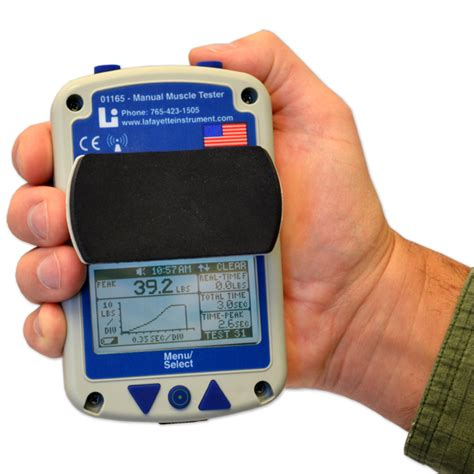
\includegraphics[width=0.4\textwidth]{figure/lafayette_01165a.jpeg}
  \caption{Lafayette 01165A Hand-Held Dynamometer}
  \label{fig:lafayette_hhd}
\end{figure}

Though not universally available in all clinical settings, hand-held dynamometry represents an evidence-informed extension of manual muscle testing. It is particularly useful for documenting progress, informing prognosis, and supporting return-to-activity decisions.

\begin{labactivitybox}
\textbf{Activity: MMT Application Across Planes and Conditions}

You will perform focused testing on two assigned motions:

\begin{itemize}
  \item \textbf{Shoulder abduction} (frontal plane)
  \item \textbf{Hip flexion} (sagittal plane)
\end{itemize}

For each movement, perform the following:

\begin{enumerate}
  \item Position your partner for a gravity-resisted MMT.
  \item Apply a standard \textbf{break test}, observing stabilization and effort.
  \item Repeat the test using the \textbf{Lafayette 01165A Hand-Held Dynamometer} to measure peak force.
  \item Reposition your partner for a \textbf{gravity-eliminated} MMT and reassess the motion.
\end{enumerate}

\textit{Record:}
\begin{itemize}
  \item Which muscles are primarily responsible for producing the movement?
  \item Which test position best allowed you to observe the muscle’s contribution?
  \item How did the resistance application and observed strength differ across test conditions?
  \item What were the practical challenges of using the dynamometer?
  \item Compare performance between the two movements. Were differences more pronounced in break test, gravity-eliminated testing, or HHD force output?
  \item \textbf{Note:} In future labs, you’ll also be responsible for identifying each muscle’s peripheral nerve and most common spinal root(s); as well as how the stabilizers and muscle length of antagonists can influence test results. Use this opportunity to start developing that habit of reasoning.
\end{itemize}
\end{labactivitybox}

\section*{Muscle Length Testing (MLT)}

\subsection*{Purpose}
Muscle length testing is used to determine whether a muscle (including its surrounding connective tissue) can lengthen sufficiently to allow normal joint motion and posture. It helps identify if a muscle is functionally \textbf{limited} (shortened), \textbf{normal}, or \textbf{excessive} (over-lengthened). A shortened muscle may restrict motion, contribute to stiffness, or drive compensatory movement patterns. 

\subsection*{Conceptual Basis}

Muscle length is typically assessed by evaluating the range of motion (ROM) permitted at the joint and reasoning about possible causes if ROM is reduced. Muscle length is one possible reason for reduced ROM (you'll review others in the Osteology \& Arthrology Lab). While this is often expressed in degrees of joint motion, it reflects the extensibility and resting tension of the muscle-tendon unit, not just joint mechanics. Muscle length limitations are particularly common in muscles that lengthen across more than one joint.

\subsubsection*{Passive Insufficiency and Length Testing}

Many special tests for muscle length target multiarticular muscles because of the clear influence of \textbf{passive insufficiency}\footnote{See Chapter 3 of \textit{Clinical Physiology: A Muscle-Centered Approach} for a detailed explanation of passive insufficiency and the length–tension properties of muscle-tendon units.}. This occurs when a muscle cannot lengthen enough to allow acceptable joint excursion at all of the joints crossed by the muscle, such as the hamstrings during combined hip flexion and knee extension. Recognizing passive insufficiency is essential for interpreting muscle length in functional movement.

\subsection*{Testing Procedure}

\begin{itemize}
  \item \textbf{Patient Positioning:} Choose a position—supine, prone, side-lying, or seated—that best exposes the muscle to be lengthened while minimizing compensatory movement.

  \item \textbf{Order of Lengthening:} To assess muscle length, position the patient so that the muscle is elongated across all the joints it spans. This typically involves moving the joints in the direction opposite to the muscle’s action—starting with the joint closest to the muscle’s origin and progressing toward the joint nearest its insertion. For example, when testing the hamstrings, begin by flexing the hip and then extending the knee. This sequence ensures a controlled, functional stretch of the muscle-tendon unit.

  \item \textbf{Tissue Resistance Points:}
    \begin{itemize}
      \item \textbf{R1 (First Resistance):} The first perceptible increase in tissue tension, which may limit available motion or alter control.
      \item \textbf{R2 (Second Resistance):} The end of available range, marked by a firm stop, compensatory motion, or discomfort.
    \end{itemize}

  \item \textbf{Observation:} Monitor for substitution patterns such as pelvic tilt, spinal shift, scapular elevation, or altered joint mechanics, which suggest compensation or movement limitation.

  \item \textbf{Determination:} Based on range, tissue resistance, and symmetry with the opposite side, classify the muscle length as \textbf{Limited}, \textbf{Normal}, or \textbf{Excessive}.
\end{itemize}

\subsection*{Clinical Context}
MLT findings should always be interpreted in the context of functional movement patterns. A muscle that appears long may in fact be under-recruited or inhibited; one that is short may be overactive or stiff. MLT, like MMT, is hypothesis-generating and should be integrated with movement observation and neurovascular examination.

\begin{labactivitybox}
\textbf{Activity: Rectus Femoris Muscle Length Testing – Modified Thomas Test}

This activity guides you through assessment of the rectus femoris using a proximal-to-distal joint sequencing strategy, consistent with standard testing logic.

\textbf{Procedure:}
\begin{itemize}
  \item Position the patient supine at the edge of the table, holding one knee to the chest.
  \item Allow the test leg to drop into hip extension.
  \item Passively flex the knee to assess length, observing for R1 (initial resistance), R2 (firm end-range), and any compensations (e.g., pelvic tilt).
\end{itemize}

\textbf{Clinical Note:} This test follows the typical “proximal to distal” sequence (hip extension then knee flexion), aligning with common instructional frameworks.

\textit{Record:}
\begin{itemize}
  \item When did R1 and R2 occur?
  \item What compensations were observed?
  \item Classify length as \textbf{Limited}, \textbf{Normal}, or \textbf{Excessive}.
  \item Was the result symmetrical between limbs?
\end{itemize}
\end{labactivitybox}

\begin{labactivitybox}
\textbf{Activity: Hamstring Muscle Length Testing – Straight Leg Raise (SLR)}

This activity evaluates hamstring length using the passive straight leg raise. This common clinical test reverses the typical joint sequencing heuristic.

\textbf{Procedure:}
\begin{itemize}
  \item Position the patient supine with the non-test leg flat.
  \item Passively flex the hip with the test knee extended.
  \item Observe for R1, R2, and any compensatory movements (e.g., posterior pelvic tilt, lumbar flattening).
\end{itemize}

\textbf{Clinical Note:} Unlike standard sequencing, this test proceeds distal-to-proximal (knee extended, then hip flexed). Consider how this reversal influences your interpretation of passive insufficiency.

\textit{Record:}
\begin{itemize}
  \item When did R1 and R2 occur?
  \item What compensations were observed?
  \item Classify length as \textbf{Limited}, \textbf{Normal}, or \textbf{Excessive}.
  \item Was the result symmetrical between limbs?
  \item \textbf{Reflection:} How might you modify this test to follow a proximal-to-distal sequence? Would that improve or hinder interpretation?
\end{itemize}
\end{labactivitybox}

\section*{Clinical Integration}

\begin{itemize}
  \item How does functional movement screening (e.g., SFMA Top Tier) inform your selection of specific MMT or MLT procedures?
  \item What are the limitations of MMT and MLT when interpreted in isolation? How do you begin to reason through cause vs. compensation?
  \item Where did you observe passive or active insufficiency? How did it affect your interpretation of muscle function?
  \item How might the results of these tests guide further investigation (e.g., reflex testing, palpation, RUSI)?
\end{itemize}

\section*{Next Steps}

\begin{itemize}
  \item Review the principles of manual muscle and length testing, with attention to test positioning, stabilization, and resistance application.
  \item Practice MMT and MLT procedures for the hamstrings and rectus femoris during Open Lab or Recitation as review of the underlying principles (you'll be doing these tests again when we get to pelvis/hip).
  \item Begin reviewing innervation (peripheral nerve and nerve root) for the muscles you tested, as this will be central to Week 2.
  \item Preview Chapter 3 in \textit{Clinical Physiology: A Muscle-Centered Approach} to reinforce your understanding of the length–tension relationship and insufficiency patterns (we'll be covering it next week in Clinical Physiology anyway).
\end{itemize}

\section*{Checklist Summary}

\begin{itemize}
  \item [$\square$] Performed and interpreted SFMA Top Tier patterns, with identification of major muscle contributors.
  \item [$\square$] Conducted gravity-resisted MMT for hip flexion and shoulder abduction, with break test and HHD measurement.
  \item [$\square$] Performed gravity-eliminated MMT for one assigned motion, using appropriate positioning and stabilization.
  \item [$\square$] Documented primary movers, observed strength, and compensation patterns for MMT scenarios.
  \item [$\square$] Conducted modified Thomas test and interpreted rectus femoris length, including R1, R2, and observed compensations.
  \item [$\square$] Conducted straight leg raise (SLR) for hamstrings, with R1, R2, and interpretation of sequencing and compensations.
\end{itemize}

% !TEX root = ../notes_template.tex
\chapter{Intro to Reflexes, Pulses \& RUSI}\label{chp:reflex_pulse}

\section*{Objectives}

By the end of this week’s lab, you will be able to:

\begin{itemize}
  \item Demonstrate proper technique for eliciting deep tendon reflexes (DTRs) and interpret findings using the 0–4+ grading scale.
  \item Correlate reflex findings with segmental innervation and Week 1 muscle testing results.
  \item Identify the “5 Ps” of ultrasound scanning and demonstrate basic probe handling techniques.
  \item Distinguish echogenic properties of soft tissues and recognize common musculoskeletal ultrasound signatures.
  \item Acquire and interpret basic B-mode ultrasound images of the patellar tendon and long head of the biceps.
  \item Compare palpated pulses with corresponding ultrasound imaging to assess vascular anatomy and perfusion.
\end{itemize}

\section*{Overview}
This week focuses on examining segmental neurology and vascular supply through deep tendon reflexes (DTR), pulse palpation, and rehabilitation ultrasound imaging. These tools build upon Week 1’s muscle testing by offering complementary insights into motor output, neurovascular status, and muscle activation.

\section*{Deep Tendon Reflex Testing (DTR)}

\subsection*{Purpose and Segmental Relevance}

Deep tendon reflexes (DTRs) provide a rapid screen of the integrity of the spinal reflex arc and can support localization of neurological findings. When interpreted alongside MMT, they offer insight into the potential cause of muscle weakness. A \textbf{diminished or absent reflex} may suggest lower motor neuron (LMN) involvement, such as dysfunction at the nerve root or peripheral nerve. In contrast, an \textbf{exaggerated or brisk reflex} may indicate upper motor neuron (UMN) involvement, typically reflecting central nervous system dysfunction above the spinal reflex level.

This week, you will assess two reflexes that correspond to previously tested muscles:

\begin{itemize}
  \item \textbf{Biceps Reflex}
  \begin{itemize}
    \item \textbf{Nerve Roots:} C5–C6
    \item \textbf{Peripheral Nerve:} Musculocutaneous
  \end{itemize}

  \item \textbf{Patellar Reflex}
  \begin{itemize}
    \item \textbf{Nerve Roots:} L3–L4
    \item \textbf{Peripheral Nerve:} Femoral
  \end{itemize}
\end{itemize}

\subsection*{General Guidelines for Reflex Testing}

Effective reflex testing requires both proper setup and refined technique. Follow these guidelines to elicit accurate and interpretable responses:

\begin{itemize}
  \item \textbf{Position the patient:} The limb being tested should be relaxed and partially supported. Use a gravity-neutral position when possible.
  \item \textbf{Identify the tendon:} Palpate and locate the tendon to be tapped. If needed, slightly stretch the tendon to increase responsiveness.
  \item \textbf{Stabilize the segment:} Use your non-dominant hand to support or stabilize the proximal joint without tension.
  \item \textbf{Use a quick wrist motion:} Tap the tendon briskly with a reflex hammer, using a relaxed wrist and smooth follow-through.
  \item \textbf{Observe the response:} Look for the muscle’s immediate contraction—not just limb movement. Repeat 2–3 times if needed.
  \item \textbf{Compare bilaterally:} Always test both sides to assess symmetry and establish a functional baseline.
\end{itemize}

\subsection*{Grading and Interpretation}

Reflexes are graded on a standardized 0–4+ scale:

\begin{itemize}
  \item \textbf{0:} Absent (areflexia)
  \item \textbf{1+:} Diminished (hyporeflexia)
  \item \textbf{2+:} Normal
  \item \textbf{3+:} Brisk (may be normal or early hyperreflexia)
  \item \textbf{4+:} Clonus (sustained reflex activity; pathological)
\end{itemize}

\textit{Interpretation Tip:} A reduced or absent reflex may indicate a peripheral or lower motor neuron lesion. A brisk or exaggerated reflex may point toward an upper motor neuron lesion.

\begin{labactivitybox}
\textbf{Activity: Segmental Reflex Screening – Biceps and Patellar}

Perform and grade the biceps and patellar reflexes on both limbs. Use your Week 1 MMT findings to inform your interpretation.

\textit{Record:}
\begin{itemize}
  \item Reflex grade (0–4+) for each limb.
  \item Is the response symmetrical?
  \item Does the reflex correlate with your MMT findings?
  \item What would a hypo- or hyper-reflexive finding suggest?
\end{itemize}
\end{labactivitybox}

\section*{Introduction to Rehabilitative Ultrasound Imaging (RUSI)}

Rehabilitative Ultrasound Imaging (RUSI) allows real-time visualization of soft tissue structures to support functional assessment and therapeutic reasoning. Unlike diagnostic imaging, which aims to detect pathology, RUSI augments a physical therapist’s clinical reasoning by enabling observation of muscle contraction, tendon morphology, fascial continuity, and spatial relationships during clinical tasks and dynamic movement.\footnote{Conceptual framework adapted from Teyhen et al. (2007), \textit{Rehabilitative Ultrasound Imaging}; technical notes adapted from Coppola, S. DPT (2024), \textit{Diagnostic Ultrasound Notes}.}

\section*{Introduction to Rehabilitative Ultrasound Imaging (RUSI)}

Rehabilitative Ultrasound Imaging (RUSI) allows real-time visualization of soft tissue structures to support functional assessment and therapeutic reasoning. Unlike diagnostic ultrasound imaging, which aims to detect pathology, RUSI augments a physical therapist’s clinical reasoning by enabling observation of muscle contraction, tendon morphology, fascial continuity, and spatial relationships during clinical tasks and dynamic movement.\footnote{Conceptual framework adapted from Teyhen et al. (2007), \textit{Rehabilitative Ultrasound Imaging}; technical notes adapted from Coppola, S. DPT (2024), \textit{Diagnostic Ultrasound Notes}.}

\subsection*{Fundamentals of Ultrasound Imaging}

\begin{itemize}
  \item \textbf{Probe Type:} We will mostly use a \textbf{linear transducer} (7–15 MHz) optimal for superficial musculoskeletal structures.

  \item \textbf{Probe Orientation:} 
  \begin{itemize}
    \item \textbf{Long Axis (LAX):} Indicator toward head — left side of screen is cephalad.
    \item \textbf{Short Axis (SAX):} Indicator to patient’s right — left side of screen is lateral.
  \end{itemize}

  When the probe is held perpendicular to the surface, the ultrasound machine generates a real-time “slice” of the anatomy immediately beneath it. In \textbf{Long Axis (LAX)}, the image represents a longitudinal view—like looking along the length of a muscle or tendon. In \textbf{Short Axis (SAX)}, the image is a transverse cross-section of the structures. The structures seen on screen represent only that specific 2D imaging plane under the probe.

  \item \textbf{Image Modes:} B-mode (brightness mode) creates grayscale cross-sectional images from echo amplitudes.

  \item \textbf{Key Settings:} 
  \begin{itemize}
    \item \textbf{Depth} — adjust to position of target structure.
    \item \textbf{Gain} — controls brightness uniformly.
    \item \textbf{TGC} (Time Gain Compensation) — adjusts brightness at different depths.
  \end{itemize}
\end{itemize}

\begin{figure}[H]
\centering
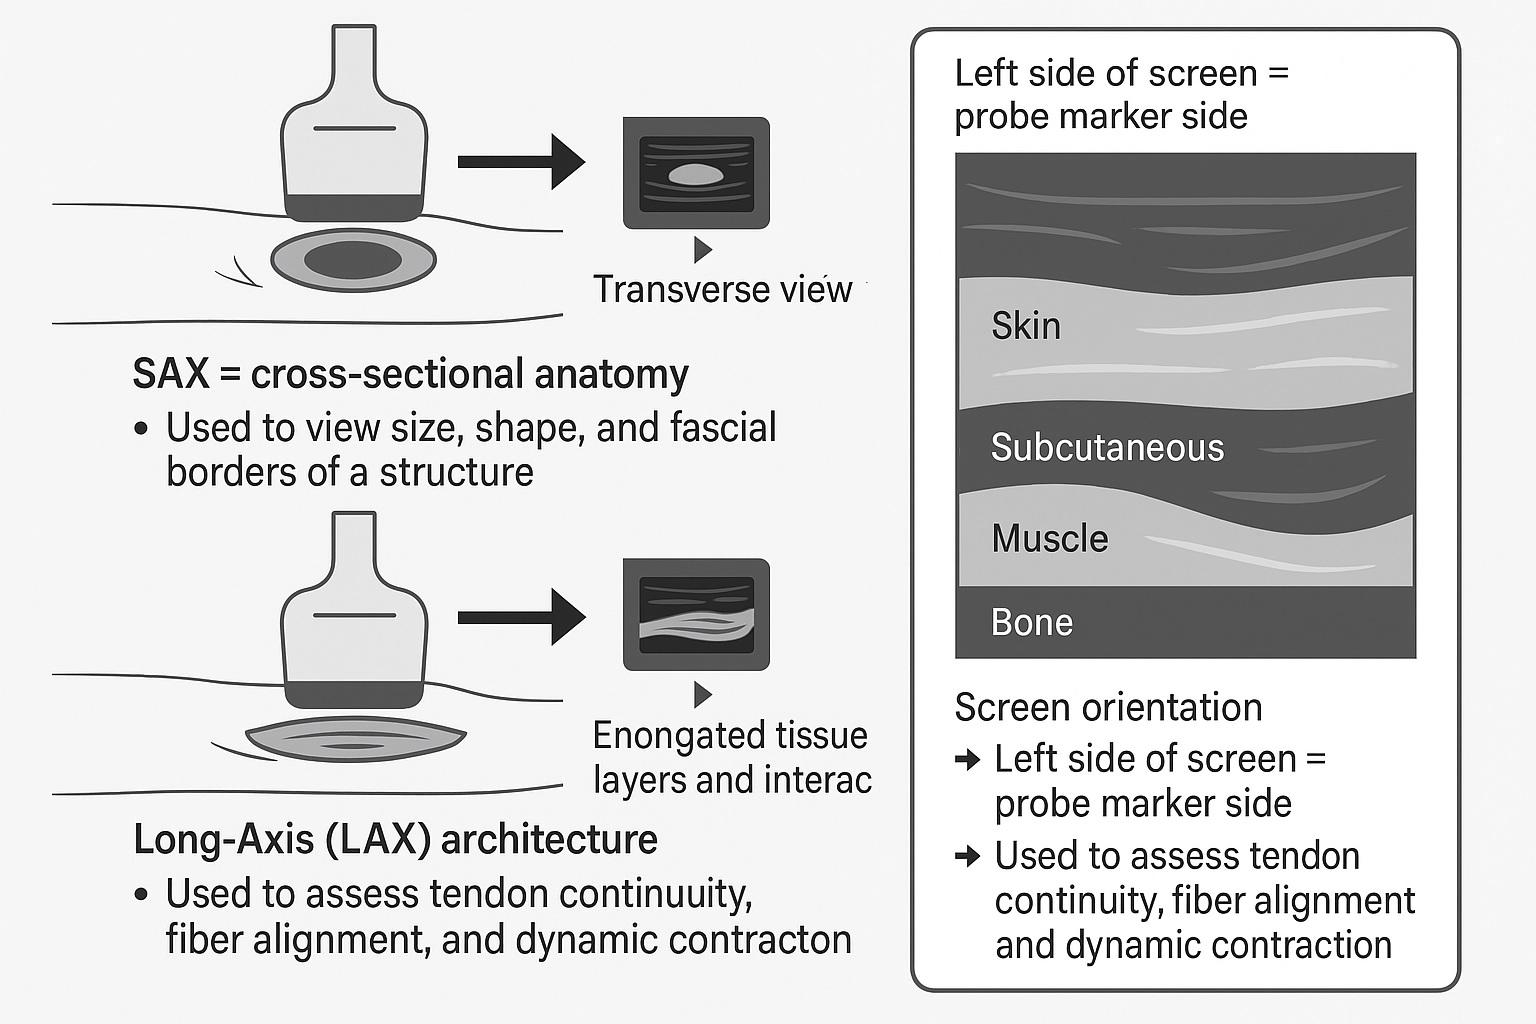
\includegraphics[width=0.75\textwidth]{figure/ultrasound_probe_orientation.png}
\caption{Schematic visualization of ultrasound probe placement: Short-Axis (SAX) and Long-Axis (LAX) views. Arrows indicate the path of the sound beam and screen orientation. This convention is foundational for interpreting RUSI scans across multiple anatomical regions.}
\label{fig:probe_orientation}
\end{figure}

\subsection*{Understanding Echogenicity}

Echogenicity refers to the ability of a tissue to reflect ultrasound waves and appear on the screen as varying shades of brightness:

\begin{itemize}
  \item \textbf{Hyperechoic:} Tissues that reflect many sound waves, appearing bright or white (e.g., bone, tendon).
  \item \textbf{Hypoechoic:} Tissues that reflect fewer sound waves, appearing darker gray (e.g., muscle).
  \item \textbf{Anechoic:} Structures that do not reflect sound waves, appearing completely black (e.g., blood-filled vessels).
\end{itemize}

\subsection*{Tissue Signatures on Ultrasound}

\begin{itemize}
  \item \textbf{Muscle (LAX):} Feather-like hypoechoic bundles with hyperechoic septa.
  \item \textbf{Tendon (LAX):} Bright, fibrous, striated appearance; more echogenic than muscle.
  \item \textbf{Nerve (SAX):} “Honeycomb” pattern — hypoechoic fascicles with hyperechoic boundaries.
  \item \textbf{Bone:} Continuous hyperechoic line with posterior shadowing.
  \item \textbf{Vessels:} Anechoic circles; arteries are pulsatile and non-compressible, veins compress with pressure.
\end{itemize}

\subsection*{Anisotropy}

Anisotropy refers to the angle-dependent appearance of certain tissues on ultrasound—particularly tendons and nerves. These structures are highly reflective when the sound waves strike them at a perpendicular angle. If the probe is slightly tilted (not perpendicular), the returning echoes are diminished, and the structure appears falsely dark (hypoechoic).

\textbf{Clinical Implication:} A healthy tendon may appear pathologically dark if scanned at a poor angle. To correct for anisotropy, use heel-toe adjustments or fine probe tilting to maintain a perpendicular beam. This technique is especially important when imaging linear structures like the patellar tendon or long head of biceps.

\subsection*{The 5 Ps of Ultrasound Scanning}

To support consistent scanning performance, this lab uses the “5 Ps” framework developed by Coppola, S. DPT (2024):\footnote{Adapted from Coppola, S. DPT (2024), \textit{Diagnostic Ultrasound Notes}.}

\begin{itemize}
  \item \textbf{Patient Position:} Ensure the patient is relaxed and optimally positioned for the target region.
  \item \textbf{Provider Position:} Position yourself ergonomically, with stable posture and clear visualization of the screen.
  \item \textbf{Probe Position:} Align the probe with appropriate orientation (LAX or SAX), contact, and angle relative to the anatomy.
  \item \textbf{Parameters:} Adjust depth, gain, and TGC for optimal visualization of the target structure.
  \item \textbf{Picture:} Evaluate the image for clarity, contrast, and correct anatomical relationships.
\end{itemize}

\subsection*{Operational Techniques}

\begin{itemize}
  \item \textbf{Static Scanning:} Position the probe using a known bony window, minimize motion, adjust image.
  \item \textbf{Dynamic Scanning:} Incorporate movement or muscle contraction; stabilize probe and observe response.
  \item \textbf{Techniques:} Fanning, heel-toe, rotating, sliding (translation) — performed slowly with controlled pressure.
\end{itemize}

\subsection*{Describing Probe Motion Techniques}

The following probe maneuvers help optimize image clarity, alignment, and depth of field:

\begin{itemize}
  \item \textbf{Heel-Toe:} Tilting the probe on its long axis to angle the ultrasound beam inferiorly or superiorly without translation.
  \item \textbf{Fanning:} Pivoting the probe across a fixed point to scan through a structure in sequential planes (like tilting on its short axis).
  \item \textbf{Sliding (Translation):} Moving the entire probe across the skin while maintaining orientation.
  \item \textbf{Rotation:} Turning the probe about its axis to switch between long and short axis views.
\end{itemize}

\begin{figure}[H]
  \centering
  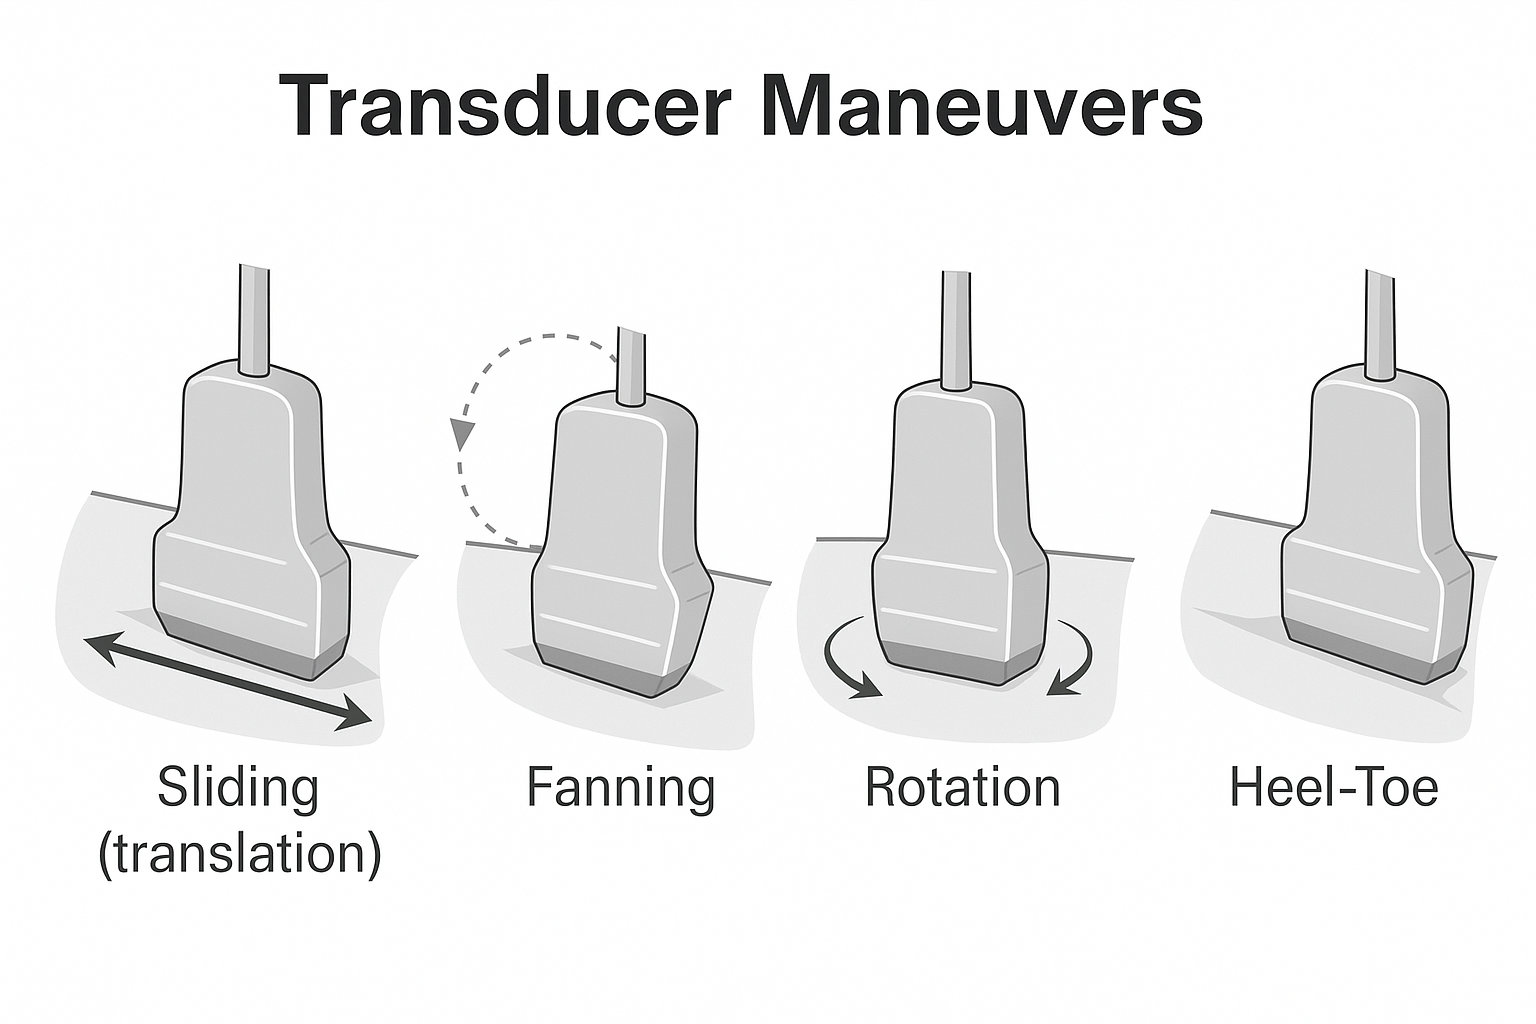
\includegraphics[width=0.6\textwidth]{figure/transducer_manuevers.png}
  \caption{Transducer manipulation techniques: Heel-Toe, Fanning, Sliding, and Rotation. Adjustments like these are essential for image clarity, anatomical accuracy, and resolving anisotropy.}
  \label{fig:transducer_maneuvers}
\end{figure}

\subsection*{Clinical Relevance in this Lab}

RUSI will be used:
\begin{itemize}
  \item To observe superficial muscle morphology (e.g., thickness, contraction, and symmetry).
  \item To assess dynamic muscle motion during voluntary contraction or positioning.
  \item To visualize vascular structures and assess pulse presence, especially when distal perfusion is in question.
\end{itemize}

\textbf{Integration Note:} As you learn RUSI, connect image interpretation with your anatomical palpation, movement analysis, and neural tracing skills. This is not an isolated tool—it is a window into functional anatomy in motion.

\medskip

\subsection*{RUSI Lab Activities}

\begin{labactivitybox}
\textbf{Activity: RUSI Session 1 – Patellar Tendon}

Use a linear transducer to visualize the patellar tendon in long axis (LAX) and short axis (SAX). This session emphasizes probe alignment, depth adjustment, and recognition of anisotropy.

\textit{Steps:}
\begin{enumerate}
  \item Position the patient supine with the knee extended.
  \item Palpate the patellar tendon between the inferior pole of the patella and tibial tuberosity.
  \item Place the probe in LAX and adjust depth and gain for optimal visualization.
  \item Identify the bright linear structure of the tendon and underlying hyperechoic bone with shadowing.
  \item Rotate to SAX view and confirm the round, fibrous tendon appearance.
\end{enumerate}

\textit{Record:}
\begin{itemize}
  \item Which transducer orientation yielded the clearest image of tendon structure?
  \item Was anisotropy present? How did you resolve it?
  \item What adjacent structures were visible in each view?
\end{itemize}
\end{labactivitybox}

\vspace{1em}

\begin{labactivitybox}
\textbf{Activity: RUSI Session 2 – Biceps Tendon (Long Head)}

This scan focuses on the long head of the biceps tendon in the bicipital groove, introducing layered anatomy, bony landmarks, and SAX vs. LAX confirmation.

\textit{Steps:}
\begin{enumerate}
  \item Position the patient seated with arm resting and slightly externally rotated.
  \item Identify the bicipital groove just distal to the acromion.
  \item Begin with SAX view: the tendon should appear as a bright oval structure between two bony ridges.
  \item Rotate to LAX to view the longitudinal path of the tendon toward the musculotendinous junction.
  \item Adjust for anisotropy, gain, and depth as needed.
\end{enumerate}

\textit{Record:}
\begin{itemize}
  \item How did the bony landmarks help guide your probe orientation?
  \item Which artifacts were present, and how were they addressed?
  \item How does this imaging reinforce your palpation and anatomical understanding from Week 1?
\end{itemize}
\end{labactivitybox}

\section*{Pulse Palpation}

\subsection*{Clinical Significance of Pulse Palpation in Muscle Assessment}

Palpating a peripheral pulse is not only about identifying cardiovascular health; it also serves as an essential screen of local muscle perfusion. Muscle contraction and endurance rely on sufficient delivery of oxygen and nutrients through the extracellular fluid (ECF), and adequate removal of metabolic byproducts. These principles are foundational to skeletal muscle physiology and become especially relevant in cases of weakness, fatigue, or inflammation.

The capillary microcirculation within muscle is supported by systemic and regional arterial flow, and even subtle limitations in perfusion can compromise muscle performance. Thus, assessing pulse strength and symmetry provides valuable insight into possible vascular or autonomic contributions to impaired muscle function.

Ultrasound can augment this assessment by directly visualizing arterial pulsatility and compressibility in real time, reinforcing what is palpated with the hands. \footnote{Adapted from Chapters 7 and 9 of \textit{Clinical Physiology: A Muscle-Centered Approach}}

\subsection*{Palpation Augmented by Ultrasound}

Palpation of peripheral pulses is a foundational skill in assessing circulation, perfusion, and vascular integrity. While clinical practice typically relies on tactile pulse grading, ultrasound can augment this process by directly visualizing arterial pulsatility and vessel compressibility.

In this lab, you will combine manual pulse palpation with B-mode ultrasound to enhance your understanding of vascular location, depth, and response.

\textbf{Target Pulse: Radial Artery}
\begin{itemize}
  \item Located just lateral to the flexor carpi radialis tendon at the distal forearm.
  \item Best visualized in short axis with the probe placed transversely over the artery.
  \item Appears as a round, anechoic vessel; observe wall motion or use light pressure to confirm pulsatility.
\end{itemize}

\begin{labactivitybox}
\textbf{Activity: Palpating and Imaging the Radial Pulse}

\textit{Steps:}
\begin{enumerate}
  \item Palpate the radial pulse using light finger pressure on both wrists.
  \item Grade the strength of the pulse on a 0–4+ scale.
  \item Place the linear transducer transversely over the palpated site and visualize the artery.
  \item Observe real-time pulsatility and compare symmetry between sides.
  \item Apply gentle compression to assess vessel compressibility.
\end{enumerate}

\textit{Record:}
\begin{itemize}
  \item Pulse strength (0–4+) and symmetry by palpation.
  \item Was the artery visible on ultrasound? What settings or adjustments improved the image?
  \item Did ultrasound confirm your palpation findings?
  \item What was the relationship between probe angle, compression, and arterial visualization?
\end{itemize}
\end{labactivitybox}

\section*{Clinical Integration}

This week’s lab expanded the diagnostic value of manual testing by integrating reflexes, vascular assessment, and imaging. Deep tendon reflexes help clarify whether muscle weakness stems from lower motor neuron (LMN) involvement (reduced reflexes) or possible upper motor neuron (UMN) involvement (brisk or clonic reflexes). When paired with MMT, reflex findings provide additional insight into whether reduced strength may have a neural origin.

Rehabilitative ultrasound imaging (RUSI) confirmed muscle presence, morphology, and contraction symmetry—adding visual validation to your palpation and manual testing findings. Pulse palpation, augmented by imaging, emphasized the critical role of local perfusion in muscle function and endurance. Together, these tools reinforce a systems-based view of neuromuscular performance.

\section*{Next Steps}

\begin{itemize}
  \item Continue practicing reflex testing using proper positioning and grading scales.
  \item Review and reinforce the nerve root–muscle–reflex mapping introduced in Weeks 1–2.
  \item Practice RUSI techniques during open lab hours: probe stabilization, depth/gain settings, and tissue recognition.
  \item Begin previewing the upper extremity regional testing approach for Week 3, especially MMT and MLT of the shoulder girdle.
\end{itemize}

\section*{Checklist Summary}

\begin{itemize}
  \item [$\square$] Performed and graded deep tendon reflexes (DTRs) for biceps and patellar tendons, using the 0–4+ scale.
  \item [$\square$] Interpreted DTR findings in relation to muscle weakness and motor neuron involvement.
  \item [$\square$] Identified musculoskeletal tissue types (muscle, tendon, nerve, bone, vessel) on ultrasound using proper LAX and SAX orientation.
  \item [$\square$] Applied the “5 Ps” of scanning and demonstrated effective use of probe motion techniques (heel-toe, fanning, sliding, rotation).
  \item [$\square$] Acquired and interpreted B-mode ultrasound images of the patellar and biceps tendons in both LAX and SAX views.
  \item [$\square$] Visualized and confirmed the radial artery using ultrasound, assessing pulsatility and compressibility.
  \item [$\square$] Compared palpated radial pulse with ultrasound visualization, noting symmetry and vessel location.
\end{itemize}


% !TEX root = ../notes_template.tex
\chapter{Shoulder Complex}\label{chp:shoulder_complex}

\section*{Objectives}
\begin{itemize}
  \item Perform and interpret manual muscle testing (MMT) of glenohumeral and scapulothoracic musculature.
  \item Identify each tested muscle’s innervation and most common spinal root(s).
  \item Conduct focused muscle length testing (MLT) of upper quarter muscles relevant to shoulder mechanics.
  \item Palpate and image the axillary artery using ultrasound.
  \item Acquire and interpret static and dynamic rehabilitative ultrasound images of the supraspinatus tendon and AC region.
\end{itemize}

\section*{Functional Context and Movement Relevance}

The shoulder is a highly mobile region that depends on coordinated scapulohumeral rhythm for functional movement. Proper glenohumeral motion is dependent on the ability of the scapula to rotate upward to maintain congruence between the humeral head and the glenoid fossa. Dysfunction of the scapulothoracic joint often manifests itself as impaired shoulder strength, aberrant movement patterns, or compensatory postures.

This week builds directly on the functional movement lens of Week 1 by focusing on the Selective Functional Movement Assessment (SFMA) upper extremity top-tier patterns:

\begin{itemize}
  \item \textbf{UE1:} Shoulder internal rotation with extension – reach behind back.
  \item \textbf{UE2:} Shoulder external rotation with abduction – reach behind head.
\end{itemize}

These movements help reveal asymmetries, motion restrictions, and potential motor control deficits in the shoulder complex. In this lab, you'll build from these patterns to investigate glenohumeral and scapular muscle function more precisely through MMT, MLT, and ultrasound-based evaluation.

\section*{Shoulder Complex Muscles by Attachment}

\noindent
Understanding shoulder complex muscles by their anatomical attachments—whether they span from the thorax, scapula, or clavicle—helps clarify how they contribute to scapular positioning and glenohumeral motion. This organization is not only anatomically meaningful, but functionally essential when performing manual muscle testing (MMT). 

Knowing which region anchors the muscle informs both \textbf{where stabilization should occur} and \textbf{how resistance should be applied} to bias the target muscle. For example, testing a thoracoscapular muscle like the rhomboids requires stabilizing the thorax and observing scapular movement, whereas testing a scapulohumeral muscle like the deltoid focuses on glenohumeral motion with attention to scapular positioning. This attachment-based framework supports more accurate test setup, interpretation, and clinical reasoning.

\vspace{.5cm}

\begin{tabular}{|p{4.5cm}|p{4.5cm}|p{5cm}|}
\hline
\textbf{Thoracoscapular} & \textbf{Thoracohumeral} & \textbf{Scapulohumeral} \\
\hline
Trapezius &
Latissimus Dorsi &
Deltoid  \\
Serratus Anterior &
Pectoralis Major &
Supraspinatus \\
Rhomboid Major &
 &
Infraspinatus \\
Rhomboid Minor &
 &
Subscapularis \\
Levator Scapulae &
 &
Teres Minor \\
Pectoralis Minor &
 &
Teres Major \\
Subclavius &
 &
Biceps Brachii  \\
 &
 &
Triceps Brachii (long head) \\
\hline
\end{tabular}

\section*{Scapular Movements: Muscles and Innervation}

\vspace{.5cm}

\noindent
The table below organizes scapular osteokinematic movement patterns by their primary muscular contributors (synergists for the motion), along with each muscle’s peripheral nerve and most common nerve root(s). Muscles are grouped by movement and listed top-down by ascending nerve root to aid in clinical reasoning and motor screening.

\begin{tabular}{|p{4cm}|p{4.5cm}|p{4cm}|p{2.5cm}|}
\hline
\textbf{Scapular Motion} & \textbf{Muscle} & \textbf{Peripheral Nerve} & \textbf{Nerve Root(s)} \\
\hline
\multirow{3}{*}{Elevation} 
  & Levator Scapulae & Dorsal Scapular & C3–C5 \\
  & Upper Trapezius & Spinal Accessory & CN XI, C1–C5 \\
  & Rhomboid Major & Dorsal Scapular & C4–C5 \\
\hline
\multirow{3}{*}{Depression}
  & Pectoralis Minor & Medial Pectoral & C8–T1 \\
  & Latissimus Dorsi & Thoracodorsal & C6–C8 \\
  & Lower Trapezius & Spinal Accessory & CN XI, C1–C5 \\
\hline
\multirow{3}{*}{Upward Rotation}
  & Serratus Anterior & Long Thoracic & C5–C7 \\
  & Upper Trapezius & Spinal Accessory & CN XI, C1–C5 \\
  & Lower Trapezius & Spinal Accessory & CN XI, C1–C5 \\
\hline
\multirow{4}{*}{Downward Rotation}
  & Levator Scapulae & Dorsal Scapular & C3–C5 \\
  & Rhomboid Minor & Dorsal Scapular & C4–C5 \\
  & Rhomboid Major & Dorsal Scapular & C4–C5 \\
  & Pectoralis Minor & Medial Pectoral & C8–T1 \\
\hline
\multirow{2}{*}{Retraction}
  & Rhomboid Major & Dorsal Scapular & C4–C5 \\
  & Middle Trapezius & Spinal Accessory & CN XI, C1–C5 \\
\hline
\multirow{2}{*}{Protraction}
  & Serratus Anterior & Long Thoracic & C5–C7 \\
  & Pectoralis Minor & Medial Pectoral & C8–T1 \\
\hline
\end{tabular}

\begin{tcolorbox}[colback=gray!5, colframe=black, title={Reminder: Movement, Not Muscle Isolation}]
Manual muscle testing of the shoulder complex emphasizes movements, not isolated muscles. While positioning and resistance can bias certain muscles, remember that each test reflects the performance of a movement system involving synergists, stabilizers, and coordinated motor control. Use the tables above to inform your testing, but interpret findings within the broader functional context of scapulohumeral rhythm and regional interdependence.
\end{tcolorbox}

\begin{labactivitybox}
\textbf{Activity: Scapular MMT}
\begin{itemize}
  \item Test scapular elevation, depression, protraction, retraction, and upward/downward rotation.
  \item Document observed compensation and stabilization strategies.
  \item Identify peripheral nerve and root level for each primary muscle tested.
\end{itemize}
\end{labactivitybox}

\begin{labactivitybox}
\textbf{Activity: Muscle Length Testing of Scapulothoracic Influencers}
\begin{itemize}
  \item Perform MLT for: Pectoralis Major (sternal and clavicular heads), and Pectoralis Minor.
  \item Document R1 and R2 (points of initial and firm resistance or observed compensation).
  \item Classify each result as Limited, Normal, or Excessive based on symmetry and expected range.
\end{itemize}
\end{labactivitybox}

\section*{Glenohumeral Movements: Muscles and Innervation}

\vspace{.5cm}

\noindent
The table below organizes glenohumeral (GH) movement patterns by their primary muscular contributors, along with each muscle’s peripheral nerve and most common nerve root(s). Muscles are grouped by movement and listed top-down by ascending nerve root to support neuroanatomical reasoning.

\begin{table}[H]
\centering
\caption{Glenohumeral Joint Movements, Prime Movers, and Innervation}
\begin{tabular}{|p{4cm}|p{4.5cm}|p{4cm}|p{2.5cm}|}
\hline
\textbf{GH Movement} & \textbf{Muscle} & \textbf{Peripheral Nerve} & \textbf{Nerve Root(s)} \\
\hline
\multirow{3}{*}{Flexion}
  & Biceps Brachii & Musculocutaneous & C5–C6 \\
  & Anterior Deltoid & Axillary & C5–C6 \\
  & Coracobrachialis & Musculocutaneous & C5–C7 \\
\hline
\multirow{4}{*}{Extension}
  & Teres Major & Subscapular (low) & C5–C6 \\
  & Posterior Deltoid & Axillary & C5–C6 \\
  & Latissimus Dorsi & Thoracodorsal & C6–C8 \\
  & Triceps Brachii (lh) & Radial & C6–C8 \\
\hline
\multirow{2}{*}{Abduction}
  & Supraspinatus & Suprascapular & C5–C6 \\
  & Middle Deltoid & Axillary & C5–C6 \\
\hline
\multirow{3}{*}{Adduction}
  & Teres Major & Subscapular (low) & C5–C6 \\
  & Latissimus Dorsi & Thoracodorsal & C6–C8 \\
  & Pectoralis Major & Pectoral (med \& lat) & C5–T1 \\
\hline
\multirow{3}{*}{External Rotation}
  & Infraspinatus & Suprascapular & C5–C6 \\
  & Teres Minor & Axillary & C5–C6 \\
  & Supraspinatus\textsuperscript{1} & Suprascapular & C5–C6 \\
\hline
\multirow{4}{*}{Internal Rotation}
  & Subscapularis & Subscapular (up \& low) & C5–C6 \\
  & Teres Major & Subscapular (low) & C5–C6 \\
  & Latissimus Dorsi & Thoracodorsal & C6–C8 \\
  & Pectoralis Major & Pectoral (med \& lat) & C5–T1 \\
\hline
\end{tabular}
\end{table}

\footnotetext[1]{The supraspinatus is not a primary external rotator, but may contribute minimally to ER torque in some positions. Its primary functions are initiating abduction and compressing the humeral head. Clinically, it is often recruited during ER-focused rehab tasks due to its role in joint stability, not due to direct ER torque production.}

\begin{tcolorbox}[colback=gray!5, colframe=black, title={Final Reminder: Movement, Not Muscle Isolation}]
Manual muscle testing of the shoulder complex emphasizes movements, not isolated muscles. While positioning and resistance can bias certain muscles, remember that each test reflects the performance of a movement system involving synergists, stabilizers, and coordinated motor control. Use the tables above to inform your testing, but interpret findings within the broader functional context of scapulohumeral rhythm and regional interdependence.
\end{tcolorbox}


\begin{labactivitybox}
\textbf{Activity: Glenohumeral MMT}
\begin{itemize}
  \item Perform gravity-resisted and gravity-eliminated testing for the GH motions.
  \item Apply break test and record HHD output for one motion.
  \item Identify innervation and nerve root(s) for each muscle tested.
\end{itemize}
\end{labactivitybox}

\begin{labactivitybox}
\textbf{Activity: Muscle Length Testing of GH Influencers}
\begin{itemize}
  \item Perform muscle length tests for: Pectoralis Major (sternal/clavicular), Pectoralis Minor, Latissimus Dorsi, and Teres Major.
  \item Record R1 and R2 compensations and classify each as Limited, Normal, or Excessive.
\end{itemize}
\end{labactivitybox}


\section*{Rehabilitative Ultrasound Imaging (RUSI) of the Glenohumeral Complex}

Ultrasound imaging of the shoulder offers a unique opportunity to visualize superficial structures relevant to both movement and clinical dysfunction. In this lab, RUSI is used not to diagnose pathology, but to:

\begin{itemize}
  \item Reinforce layered anatomical relationships through real-time visualization.
  \item Practice probe handling, alignment, and anisotropy correction in a high-utility region.
  \item Identify landmarks and dynamic tissue interactions during functional shoulder motion.
\end{itemize}

The glenohumeral joint is a prime region for developing RUSI skills due to the accessibility of key tendons, the clinical relevance of shoulder dysfunction, and the well-established sonographic windows for the biceps tendon and supraspinatus outlet.

The following scans focus on clinically useful structures:
\begin{itemize}
  \item The long head of the biceps tendon — a foundational scan for shoulder RUSI orientation.
  \item The supraspinatus tendon in SAX and LAX — for assessment of tendon integrity and depth relationships.
  \item A dynamic view of the subacromial space during abduction — to explore potential impingement mechanisms.
\end{itemize}

\footnotetext{Adapted from: Collebrusco et al. (2017), \textit{The Use of Ultrasound Images in Manual Therapy}; and Bailey et al. (2015), \textit{Current Rehabilitation Applications for Shoulder Ultrasound Imaging}.}

\begin{labactivitybox}
\textbf{Activity: Biceps Tendon (Long Head) – Revisited for Shoulder Orientation}

This scan revisits the long head of the biceps tendon as a foundational reference for shoulder RUSI. Its central location within the bicipital groove provides a key landmark for orienting future scans of the rotator cuff and shoulder joint.

\textit{Steps:}
\begin{enumerate}
  \item Position the patient seated, arm relaxed and slightly externally rotated.
  \item Palpate and locate the bicipital groove just inferior to the anterior acromion.
  \item Begin with the \textbf{short axis (SAX)} view: the tendon should appear as a well-defined hyperechoic oval bordered by the greater and lesser tubercles.
  \item Rotate the probe 90° to obtain the \textbf{long axis (LAX)} view: observe the continuity of the tendon along its proximal-to-distal path.
  \item Optimize \textbf{anisotropy correction} through heel-toe adjustments, and refine image clarity with gain and depth settings.
\end{enumerate}

\textit{Record:}
\begin{itemize}
  \item What bony landmarks helped confirm SAX and LAX views?
  \item Were tendon borders clearly visualized? If not, how did you adjust probe orientation?
  \item How does this scan reinforce your anatomical model of the anterior shoulder?
  \item How might you use this position to pivot toward supraspinatus or subscapularis imaging?
\end{itemize}
\end{labactivitybox}

\begin{labactivitybox}
\textbf{Activity: Supraspinatus Tendon Imaging (Static and Dynamic)}

This scan introduces the supraspinatus tendon and the subacromial space in both SAX and LAX views, highlighting its relationship to the humeral head, greater tuberosity, acromion, and subdeltoid bursa. It includes a dynamic screen for anterior impingement.

\textit{Steps (Static Imaging):}
\begin{enumerate}
  \item Position the patient seated with the hand behind the back or on the thigh, shoulder slightly extended.
  \item \textbf{SAX View:} Place the probe transversely just anterolateral to the acromion to visualize the convex humeral head (red outline), overlying supraspinatus tendon (“tire” appearance), and subdeltoid bursa (black hypoechoic interface).
  \item \textbf{LAX View:} Rotate the probe obliquely to follow the tendon along the greater tuberosity to the musculotendinous junction. Identify a continuous, beak-shaped tendon with uniform echotexture. 
  \item Confirm tendon integrity and bursal separation from the deltoid muscle. Adjust for anisotropy.
\end{enumerate}

\textit{Steps (Dynamic Imaging for Impingement):}
\begin{enumerate}
  \item Maintain LAX orientation and passively abduct the arm from ~30° to 90°.
  \item Observe whether the supraspinatus tendon, subdeltoid bursa, or overlying deltoid compresses or narrows the acromiohumeral space.
  \item If available, use cine capture to analyze any “shearing” of the bursa during elevation.
\end{enumerate}

\textit{Record:}
\begin{itemize}
  \item Describe tendon appearance and continuity in both SAX and LAX views.
  \item Was subacromial spacing preserved or narrowed during abduction?
  \item Identify any signs of bursal impingement or deltoid encroachment.
\end{itemize}
\end{labactivitybox}

\begin{labactivitybox}
\textbf{Activity: Dynamic AC Joint Imaging – Screening for Subacromial Impingement}

This scan assesses the supraspinatus outlet and subacromial space during passive abduction to identify or rule out dynamic impingement.

\textit{Steps:}
\begin{enumerate}
  \item Place the probe in an \textbf{oblique long axis (LAX)} view over the supraspinatus tendon just inferior to the acromion.
  \item Identify the \textbf{acromion (Acr)}, \textbf{humeral head (Hum)}, and the overlying \textbf{subacromial-subdeltoid bursa}.
  \item Actively abduct the shoulder through midrange (approx. 30°–90°), keeping the probe stable.
  \item Observe for narrowing of the subacromial space, displacement or “shearing” of the tendon, or bursal effacement.
  \item Use cine loop review to assess motion patterns and tendon glide if available.
\end{enumerate}

\textit{Record:}
\begin{itemize}
  \item Was the anechoic bursal space maintained throughout abduction?
  \item Did the supraspinatus tendon deform, compress, or lose continuity under the acromion?
  \item How do these dynamic findings relate to your static supraspinatus imaging?
  \item Suggested labeling for captured loops: \texttt{Rt Ant Impng Pre} / \texttt{Post Dynamic}
\end{itemize}
\end{labactivitybox}


\section*{Pulse Palpation}

The axillary artery is the principal vascular supply to the upper extremity. As it courses beneath the clavicle and through the thoracic outlet, it is subject to compression by surrounding structures such as the scalene muscles, first rib, and pectoralis minor. This vulnerability contributes to the vascular subtype of thoracic outlet syndrome (TOS), in which mechanical compression compromises distal perfusion and contributes to symptoms such as numbness, coolness, or fatigue during upper extremity activity.

In clinical practice, assessing the axillary pulse provides insight into proximal vascular integrity. Combining palpation with RUSI enhances accuracy and reinforces anatomical understanding.

\begin{labactivitybox}
\textbf{Activity: Pulse Palpation + Imaging}
\begin{itemize}
  \item Locate and palpate the axillary pulse in a relaxed, abducted position.
  \item Image the vessel in short axis using ultrasound; assess for:
    \begin{itemize}
      \item Compressibility (vein collapses, artery remains open).
      \item Pulsatility (real-time rhythmic motion).
      \item Spatial relationships to surrounding muscles (pectoralis major/minor, deltoid).
    \end{itemize}
\end{itemize}
\end{labactivitybox}


\section*{Clinical Integration}

\begin{itemize}
  \item How did observing scapular and glenohumeral motion during movement screening influence your MMT and MLT strategy?
  \item When testing muscles around the shoulder complex, where did you find it difficult to isolate a single muscle? How did your knowledge of innervation help you interpret findings?
  \item How does the concept of regional interdependence apply to abnormal scapulohumeral rhythm or pain during shoulder movement?
  \item What role did ultrasound imaging play in reinforcing your understanding of tendon orientation and joint clearance?
  \item How did your pulse palpation findings support your understanding of the vascular anatomy of the shoulder region?
\end{itemize}

\section*{Next Steps}

\begin{itemize}
  \item Review muscle actions, innervations, and typical compensatory strategies for scapular and glenohumeral motions.
  \item Revisit the ultrasound scanning protocol for the supraspinatus and subacromial space, with attention to dynamic imaging cues.
  \item Practice shoulder MMTs with a peer, focusing on stabilization and resisting substitutions.
  \item Prepare for Week 4 by previewing distal upper extremity movements, including forearm pronation/supination and grip.
\end{itemize}

\section*{Checklist Summary}

\begin{itemize}
  \item [$\square$] Performed gravity-resisted and gravity-eliminated MMT for glenohumeral and scapular muscles.
  \item [$\square$] Identified the innervation and nerve root(s) of all muscles tested during MMT.
  \item [$\square$] Used HHD to record force output for one GH break test.
  \item [$\square$] Conducted and interpreted MLT for pectoralis major, pectoralis minor, latissimus dorsi, and teres major, including R1, R2, and compensations.
  \item [$\square$] Acquired static ultrasound images of the supraspinatus tendon in SAX and LAX.
  \item [$\square$] Performed dynamic ultrasound to assess AC joint space during shoulder abduction.
  \item [$\square$] Palpated and imaged the axillary pulse, confirming vascular characteristics via ultrasound.
\end{itemize}

% !TEX root = ../notes_template.tex
\chapter{Elbow, Forearm, Wrist \& Hand}\label{chp:distal_ue}

\section*{Objectives}
\begin{itemize}
  \item Perform and interpret MMT for elbow, forearm, wrist, hand, and thumb motions.
  \item Identify innervation and nerve root levels for each tested muscle.
  \item Conduct MLT for elbow and wrist flexor/extensor groups, including biceps and triceps brachii.
  \item Grade and interpret DTRs for the biceps and triceps tendons.
  \item Palpate and image the brachial artery using ultrasound.
  \item Observe and trace common upper extremity nerve entrapment sites using anatomical landmarks.
\end{itemize}

\section*{Peripheral Nerve Entrapment and Screening Strategy}

\noindent
Peripheral nerves can become compressed or irritated along their course, producing motor and sensory impairments distal to the entrapment. In this lab, we focus on screening for **median, ulnar, and radial** nerve integrity by combining anatomical palpation with MMT and reflex testing.

\vspace{0.5cm}

We adopt a **proximal-to-distal logic** when tracing nerves, as this mirrors both clinical reasoning and the path of nerve vulnerability. Entrapment sites are reviewed below with location cues. You will relate these sites to your testing results throughout the elbow, forearm, and hand.

\vspace{0.5cm}

\begin{table}[H]
\centering
\begin{tabular}{|p{2.8cm}|p{7cm}|p{4.7cm}|}
\hline
\textbf{Nerve} & \textbf{Entrapment Site} & \textbf{Memory Cue} \\
\hline
\multirow{4}{*}{\textbf{Median}} 
  & Bicipital Aponeurosis (anterior elbow) & “Elbow pit tunnel” \\
  & Lig of Struthers (medial distal humerus) & “Hidden elbow bridge” \\
  & Pronator Teres (proximal forearm) & “Forearm muscle trap” \\
  & Carpal Tunnel (wrist, flexor retinaculum) & “Classic compression” \\
\hline
\multirow{4}{*}{\textbf{Radial}} 
  & Radial Groove (posterior humerus) & “Humeral hug” \\
  & Radial Head (lateral elbow) & “Turning the radius” \\
  & Arcade of Frohse (edge of supinator) & “Tight supinator turn” \\
  & Supinator (deep in forearm) & “Radial squeeze” \\
\hline
\multirow{3}{*}{\textbf{Ulnar}} 
  & Arcade of Struthers (medial arm) & “Pre-cubital trap” \\
  & Cubital Tunnel (post medial epicondyle) & “Funny bone spot” \\
  & Flexor Carpi Ulnaris (between heads) & “Final tunnel” \\
\hline
\end{tabular}
\captionsetup{justification=raggedright, singlelinecheck=false}
\caption{Peripheral Nerve Entrapment Sites of the Upper Extremity (Proximal to Distal). \textit{Note: Identifying the specific location of nerve entrapment is beyond the scope of this lab and will not be assessed on the practical exam. This table is included to introduce the anatomical reasoning that underlies neuromuscular testing and to support clinical pattern recognition over time.}}
\end{table}

\section*{Elbow and Forearm Movements: Muscles and Innervation}

\vspace{.5cm}

\begin{tabular}{|p{4cm}|p{4.5cm}|p{4cm}|p{2.5cm}|}
\hline
\textbf{Movement} & \textbf{Muscle} & \textbf{Peripheral Nerve} & \textbf{Nerve Root(s)} \\
\hline
\multirow{3}{*}{Elbow Flexion}
  & Biceps Brachii & Musculocutaneous & C5–C6 \\
  & Brachialis & Musculocutaneous & C5–C6 \\
  & Brachioradialis & Radial & C5–C6 \\
\hline
Elbow Extension
  & Triceps Brachii & Radial & C6–C8 \\
\hline
Forearm Supination
  & Biceps Brachii & Musculocutaneous & C5–C6 \\
  & Supinator & Radial (deep branch) & C6–C7 \\
\hline
Forearm Pronation
  & Pronator Teres & Median & C6–C7 \\
  & Pronator Quadratus & Median  & C7–C8 \\
\hline
\end{tabular}

\begin{labactivitybox}
\textbf{Activity: MMT – Elbow and Forearm Movements}

\begin{itemize}
  \item Perform gravity-resisted and gravity-eliminated MMT for:
  \begin{itemize}
    \item Elbow flexors (biceps brachii, brachialis, brachioradialis)
    \item Elbow extensors (triceps brachii)
    \item Forearm supinators (biceps brachii, supinator)
    \item Forearm pronators (pronator teres, pronator quadratus)
  \end{itemize}
  \item Conduct a break test using the HHD for either elbow flexion or extension.
  \item Record stabilization strategies, resistance application, and observed compensatory motions.
  \item For each tested muscle, document its peripheral innervation and most common nerve root(s).
\end{itemize}
\end{labactivitybox}

\noindent Deep tendon reflex testing helps corroborate segmental integrity assessed through MMT and supports differential diagnosis of upper limb weakness.

\begin{labactivitybox}
\textbf{Activity: DTR Testing – Biceps and Triceps}

\begin{itemize}
  \item Perform reflex testing for:
  \begin{itemize}
    \item \textbf{Biceps tendon} – C5–C6 (Musculocutaneous nerve)
    \item \textbf{Triceps tendon} – C7 (Radial nerve)
  \end{itemize}
  \item Grade each reflex using the standard 0–4+ scale.
  \item Compare left vs. right for symmetry and amplitude.
  \item Correlate reflex findings with muscle strength results from MMT.
\end{itemize}
\end{labactivitybox}

\begin{labactivitybox}
\textbf{Activity: Muscle Length Testing – Upper Limb (Elbow)}
\begin{itemize}
  \item Muscles: Biceps brachii, Triceps brachii
  \item Document R1, R2, and classify muscle length.
\end{itemize}
\end{labactivitybox}


\section*{Wrist Movements: Muscles and Innervation}

\vspace{0.5cm}

\begin{tabular}{|p{4cm}|p{4.5cm}|p{4cm}|p{2.5cm}|}
\hline
\textbf{Movement} & \textbf{Muscle} & \textbf{Peripheral Nerve} & \textbf{Nerve Root(s)} \\
\hline
\multirow{2}{*}{Wrist Flexion}
  & Flexor Carpi Radialis & Median & C6–C7 \\
  & Flexor Carpi Ulnaris & Ulnar & C7–T1 \\
\hline
\multirow{2}{*}{Wrist Extension}
  & Ext Carpi Radialis Longus & Radial & C6–C7 \\
  & Extensor Carpi Ulnaris & Radial & C7–C8 \\
\hline
\multirow{2}{*}{Radial Deviation}
  & Flexor Carpi Radialis & Median & C6–C7 \\
  & Ext Carpi Radialis Longus & Radial & C6–C7 \\
\hline
\multirow{2}{*}{Ulnar Deviation}
  & Flexor Carpi Ulnaris & Ulnar & C7–T1 \\
  & Extensor Carpi Ulnaris & Radial & C7–C8 \\
\hline
\end{tabular}

\begin{labactivitybox}
\textbf{Activity: MMT – Forearm Rotation and Wrist Motion}

\begin{itemize}
  \item Test pronator teres, pronator quadratus, and supinator for forearm rotation in gravity-resisted and -eliminated positions.
  \item Test wrist flexors and extensors for strength, symmetry, and compensation.
  \item Repeat one test using HHD.
  \item Identify and record innervation and spinal root levels for each muscle.
\end{itemize}
\end{labactivitybox}

\section*{Hand Extrinsic Muscles (Gross Motor Screening Focus)}

\noindent
For clinical screening and gross motor assessment, we focus on muscle groups with functional or neurodiagnostic relevance. This includes composite grip function and selected muscles innervated by each major nerve (median, ulnar, radial).

\begin{table}[H]
\centering
\captionsetup{justification=raggedright, singlelinecheck=false}
\begin{tabular}{|p{4cm}|p{4.5cm}|p{4cm}|p{2.5cm}|}
\hline
\textbf{Movement} & \textbf{Muscle} & \textbf{Peripheral Nerve} & \textbf{Nerve Root(s)} \\
\hline
\multirow{3}{*}{Grip} 
  & FDS & Median & C7–T1 \\
  & FDP (lat. 2–3) & Median & C8–T1 \\
  & FDP (med. 4–5) & Ulnar & C8–T1 \\
\hline
MCP Ext (digits 2–5)
  & Extensor Digitorum & Radial & C7–C8 \\
\hline
\end{tabular}
\caption{\textit{Note: Grip strength primarily reflects extrinsic flexors but is also influenced by intrinsic hand muscles such as interossei and thenar muscles.}}
\end{table}

\vspace{0.5cm}

\begin{labactivitybox}
\textbf{Activity: MMT – Gross Motor Screening of Hand Function with Functional Grip Testing}

\begin{itemize}
  \item Perform \textbf{hand grip testing} using a dynamometer in three positions:
  \begin{enumerate}
    \item Neutral wrist
    \item Wrist extension (20–30°)
    \item Wrist flexion (45°)
  \end{enumerate}
  \item Compare force output and interpret differences using principles of:
  \begin{itemize}
    \item \textbf{Active Insufficiency} – wrist flexors (grip force ↓ in wrist flexion)
    \item \textbf{Passive Insufficiency} – wrist extensors (tension limits grip in wrist extension)
  \end{itemize}
  \item Manually test:
    \begin{itemize}
      \item \textbf{Extensor Digitorum} – radial nerve screen
      \item \textbf{FDP digits 4–5} – ulnar nerve screen
    \end{itemize}
  \item Record findings and note any weakness, asymmetry, or compensatory patterns.
  \item Document the peripheral nerve and spinal root(s) for each muscle tested.
\end{itemize}
\end{labactivitybox}


\section*{Hand Intrinsic Muscles (Screening Focus)}

\noindent
These intrinsic muscles are emphasized for clinical screening due to their role in functional grip and their diagnostic utility in assessing median and ulnar nerve integrity.

\begin{table}[H]
\centering
\captionsetup{justification=raggedright, singlelinecheck=false}
\begin{tabular}{|p{4cm}|p{4.5cm}|p{4cm}|p{2.5cm}|}
\hline
\textbf{Movement} & \textbf{Muscle} & \textbf{Peripheral Nerve} & \textbf{Nerve Root(s)} \\
\hline
Thumb Abduction
  & Abductor Pollicis Brevis & Median & C8–T1 \\
\hline
Thumb Adduction
  & Adductor Pollicis & Ulnar & C8–T1 \\
\hline
Index Finger Abd
  & 1st Dorsal Interosseous & Ulnar & C8–T1 \\
\hline
Digits 3–5 Abduction
  & Dorsal Interossei (2–4) & Ulnar & C8–T1 \\
\hline
Digits 3–5 Adduction
  & Palmar Interossei (2, 4, 5) & Ulnar & C8–T1 \\
\hline
MCP Flexion + IP Extension (Digits 2–3)
  & Lumbricals 1–2 & Median & C8–T1 \\
\hline
MCP Flexion + IP Extension (Digits 4–5)
  & Lumbricals 3–4 & Ulnar & C8–T1 \\
\hline
\end{tabular}
\caption{Movements of the Hand for Functional and Neurological Screening Involving Intrinsic Muscles}
\end{table}

\vspace{0.5cm}

\begin{labactivitybox}
\textbf{Activity: MMT – Intrinsic Muscle Screening of the Hand}

\begin{itemize}
  \item Manually test:
  \begin{itemize}
    \item \textbf{Abductor Pollicis Brevis} – median nerve screen
    \item \textbf{Adductor Pollicis} – ulnar nerve screen
    \item \textbf{1st Dorsal Interosseous} – ulnar nerve screen
    \item \textbf{Digits 3–5 Abduction/Adduction} – interossei for ulnar integrity
    \item \textbf{Lumbricals} (1–2 vs. 3–4) – differential median vs. ulnar screen
  \end{itemize}
  \item Observe for:
  \begin{itemize}
    \item Atrophy of thenar and first dorsal interosseous spaces
    \item Difficulty with fine grasp or pinch
    \item Imbalance between radial and ulnar side strength
  \end{itemize}
  \item Document peripheral nerve and nerve root(s) for each muscle tested.
\end{itemize}
\end{labactivitybox}


\section*{Neurovascular Ultrasound and Palpation of the Distal Upper Extremity}

\begin{labactivitybox}
\textbf{Activity: Vascular Assessment – Brachial and Radial Arteries}

\textit{Palpation + Ultrasound Visualization}
\begin{itemize}
  \item Locate and palpate the \textbf{brachial artery} in the antecubital fossa and the \textbf{radial artery} at the wrist.
  \item Use ultrasound in SAX to confirm vessel identity through \textbf{compressibility} and \textbf{pulsatility}.
  \item Observe for surrounding structures and note any asymmetry.
  \item Record findings, image depth, and probe orientation.
\end{itemize}
\end{labactivitybox}

\begin{labactivitybox}
\textbf{Activity: Peripheral Nerve Scanning – Median and Ulnar Nerves}

\textit{RUSI Localization and Entrapment Screening}

\begin{itemize}
  \item \textbf{Median Nerve:}
  \begin{itemize}
    \item Use \textbf{SAX} at the level of the carpal tunnel (between the scaphoid and pisiform) to identify the nerve’s “honeycomb” fascicular pattern deep to the flexor retinaculum.
    \item Confirm landmarks: radius (Rad), lunate (Lun), palmaris longus (PL), flexor tendons.
    \item Use \textbf{LAX} to trace the ribbon-like hypoechoic nerve as it courses deep to PL and over the lunate.
    \item Apply dynamic imaging (thumb opposition) to confirm nerve vs. tendon identity.
  \end{itemize}

  \item \textbf{Ulnar Nerve:}
  \begin{itemize}
    \item Use \textbf{SAX} at the cubital tunnel (between the medial epicondyle and olecranon) and at Guyon’s canal (level of pisiform).
    \item Identify key landmarks: pisiform (Pis), flexor digiti minimi brevis (FDMB), ulnar artery (UA), and flexor retinaculum (FR).
    \item Visualize the ulnar nerve as a hypoechoic bundle superficial to the retinaculum and lateral to the pisiform.
    \item Confirm normal fascicular pattern and assess for swelling or distortion.
  \end{itemize}

  \item \textbf{Interpretation:}
  \begin{itemize}
    \item Note probe orientation (SAX/LAX), anatomical level, image depth, and signs of entrapment (e.g., enlargement, compression, anisotropy).
  \end{itemize}
\end{itemize}
\end{labactivitybox}

\section*{Clinical Integration}

\begin{itemize}
  \item How did gross motor screening using grip, extrinsic, and intrinsic hand muscle tests guide your clinical reasoning about nerve involvement?
  \item In what ways did your MMT findings align with or differ from your reflex testing (biceps and triceps)?
  \item What patterns of weakness or asymmetry might suggest proximal vs. distal nerve entrapment?
  \item How did ultrasound imaging of the median and ulnar nerves enhance your understanding of nerve anatomy and potential entrapment zones?
  \item How might reflex integrity and motor strength together inform a diagnosis of cervical radiculopathy versus peripheral nerve compression?
\end{itemize}

\section*{Next Steps}

\begin{itemize}
  \item Consolidate your understanding of distal upper extremity innervation by reviewing dermatomes, myotomes, and reflexes.
  \item Practice the MMT procedures introduced this week for extrinsic grip, intrinsic hand muscles, and selected nerve screens.
  \item Practice the RUSI procedures for imaging the brachial and radial arteries, and the median and ulnar nerves in SAX and LAX views.
  \item Review the anatomy of the pelvic girdle and hip to prepare for Week 5, focusing on similarities in regional interdependence logic.
\end{itemize}

\section*{Checklist Summary}

\begin{itemize}
  \item [$\square$] Performed gravity-resisted and gravity-eliminated MMT for elbow flexion, extension, supination, and pronation with correct stabilization and substitution awareness.
  \item [$\square$] Used hand-held dynamometry (HHD) to quantify force output for either elbow flexion or extension.
  \item [$\square$] Performed and graded deep tendon reflexes for the biceps (C5–C6) and triceps (C7) tendons.
  \item [$\square$] Conducted MMT for extrinsic hand function (grip, finger extension, FDP) to screen radial and ulnar nerve involvement.
  \item [$\square$] Compared grip strength with wrist in flexed vs. extended positions to evaluate influence of active and passive insufficiency.
  \item [$\square$] Conducted MMT for intrinsic hand muscles (APB, adductor pollicis, 1st dorsal interosseous, lumbricals) for differential median vs. ulnar nerve screening.
  \item [$\square$] Identified and interpreted upper extremity nerve entrapment sites from elbow to wrist using anatomical landmarks.
  \item [$\square$] Acquired and interpreted ultrasound images of the median and ulnar nerves in both SAX and LAX views using dynamic validation techniques.
  \item [$\square$] Palpated and imaged the brachial and radial arteries using ultrasound to confirm pulsatility and compressibility.
\end{itemize}


% !TEX root = ../notes_template.tex
\chapter{Pelvis \& Hip}\label{chp:pelvis_hip}

\section*{Objectives}

\begin{itemize}
  \item Describe the role of the pelvis in orienting the acetabulum and supporting femoral motion during closed and open chain tasks.
  \item Interpret SFMA Top Tier patterns (MSF, MSE, MSR, SLS, ADS) to identify hip-related movement dysfunction.
  \item Perform MMT for primary hip movements (flexion, extension, abduction, adduction, internal rotation, external rotation) with correct patient positioning and stabilization.
  \item Identify muscle group innervation and root levels using neuromechanical reasoning.
  \item Conduct muscle length testing for the hamstrings, iliopsoas, rectus femoris, and TFL/ITB using standardized protocols.
  \item Acquire and interpret RUSI images of the femoral neurovascular bundle.
  \item Classify observed findings using R1/R2 reasoning, mobility/motor control logic, and functional movement integration.
\end{itemize}

\section*{Functional Integration: Pelvis \& Hip as the Proximal Engine}

The pelvis serves as the dynamic base for femoral motion, functioning analogously to the scapula in the upper extremity. Just as the scapula positions the glenoid for effective humeral mechanics, the pelvis orients the acetabulum and stabilizes the proximal femur for forceful, efficient movement.

Movements of the pelvis are, in fact, movements of the spine—primarily the lumbar spine, though contributions from the thoracic and sacral regions may be relevant depending on posture and load. These pelvic motions (e.g., anterior tilt, rotation) will be addressed in Week 8 during the Lumbopelvic Anatomy lab.

It is important to recognize that hip movements, particularly in closed chain positions, are often coupled with pelvic and spinal motions due to kinetic chain continuity. For example, an anterior pelvic tilt (achieved with lumbar extension without changing the position of the thorax in space) in standing cannot occur without concurrent hip flexion. This coupling reflects the interdependence of segmental mobility and neuromuscular control, and underscores the need for integrated assessment strategies when evaluating hip function in functional tasks.

Hip function cannot be fully understood in isolation—it is deeply integrated with lumbopelvic control and distal alignment. Dysfunction at the hip may produce lumbar pain, pelvic asymmetry, or gait deviation, while impaired trunk or knee mechanics often constrain hip mobility.

\begin{tcolorbox}[colback=gray!5, colframe=black, title={Functional Movement Approach: Top Tier SFMA Patterns}]
SFMA patterns such as MSF, MSE, MSR, and SLS rely on coordinated pelvis–hip action. Deficits in these tests may reflect mobility limitations, length impairments, or poor motor control rooted in the lumbopelvic–hip complex. The Arms Down Squat (ADS) adds an integrated assessment of hip, knee, and ankle synergy.
\end{tcolorbox}

This week’s lab uses these patterns as entry points for deeper evaluation through manual muscle testing, muscle length assessment, and RUSI-guided observation. Our aim is to link functional movement testing to segmental neuromechanical reasoning.

\subsection*{SFMA Top Tier Patterns for Pelvic-Hip Focus}

\begin{itemize}
  \item \textbf{Multisegmental Flexion (MSF)} — Observe symmetry and depth of hip hinge; limited flexion may stem from posterior chain tightness, altered lumbo-pelvic rhythm, or hip capsule restriction.
  \item \textbf{Multisegmental Extension (MSE)} — Assess anterior hip and trunk extension; pelvic thrust or asymmetry may indicate impaired hip extension, rectus femoris tightness, or poor gluteal activation.
  \item \textbf{Multisegmental Rotation (MSR)} — View pelvic dissociation and hip rotation bias; asymmetries here may flag lumbar-pelvic-hip mobility restrictions.
  \item \textbf{Single Leg Stance (SLS)} — Detect frontal plane pelvic control; Trendelenburg signs or instability may point to abductor weakness, proprioceptive deficits, or gluteal inhibition.
  \item \textbf{Arms Down Squat (ADS)} — Assess hip, knee, and ankle coordination with arms relaxed; limited depth or pelvic asymmetry may suggest hip joint restriction, motor control deficits, or compensatory strategies from above or below.
\end{itemize}

\vspace{0.25cm}

\noindent
In practice clinicians often use functional movement observations (SFMA being one example) to guide which structures to assess further via MMT, MLT, and neurovascular screening. Consider whether findings are mobility- or motor-control-driven to apply the appropriate intervention focus.


\section*{Hip Movements: Muscles and Innervation}

\vspace{0.25cm}

\noindent
The table below lists primary hip movements with corresponding prime movers, peripheral nerves, and spinal roots. Movements are organized top-down by functional direction, with muscles listed from proximal (higher root) to distal (lower root) to aid in neurosegmental reasoning.

\begin{table}[H]
\centering
\captionsetup{justification=raggedright, singlelinecheck=false}
\begin{tabular}{|p{3.5cm}|p{5cm}|p{4cm}|p{2.5cm}|}
\hline
\textbf{Movement} & \textbf{Muscle} & \textbf{Peripheral Nerve} & \textbf{Nerve Root(s)} \\
\hline
\multirow{3}{*}{Hip Flexion}
  & Iliopsoas & Femoral / Rami (L1–L3) & L1–L3 \\
  & Rectus Femoris & Femoral & L2–L4 \\
  & Sartorius & Femoral & L2–L3 \\
\hline
\multirow{3}{*}{Hip Extension}
  & Gluteus Maximus & Inferior Gluteal & L5–S2 \\
  & Hamstrings & Sciatic & L5–S2 \\
\hline
\multirow{2}{*}{Hip Abduction}
  & Gluteus Medius & Superior Gluteal & L4–S1 \\
  & Gluteus Minimus & Superior Gluteal & L4–S1 \\
\hline
\multirow{2}{*}{Hip Adduction}
  & Adductor Longus & Obturator & L2–L4 \\
  & Adductor Magnus & Obturator / Sciatic & L2–L4 \\
\hline
\multirow{2}{*}{External Rotation}
  & Piriformis & Nerve to Piriformis & L5–S2 \\
  & Obturator Externus & Obturator & L3–L4 \\
\hline
\multirow{2}{*}{Internal Rotation}
  & Tensor Fascia Latae & Superior Gluteal & L4–S1 \\
  & Gluteus Medius (ant) & Superior Gluteal & L4–S1 \\
\hline
\end{tabular}
\caption{Primary Hip Movements and Their Neuromuscular Innervation}
\end{table}

\subsection*{MMT Hip}

\begin{labactivitybox}
\textbf{Activity: MMT – Hip Flexion and Extension}

\begin{itemize}
  \item Perform gravity-resisted and gravity-eliminated testing for:
  \begin{itemize}
    \item \textbf{Hip Flexion:} Iliopsoas, Rectus Femoris, Sartorius
    \item \textbf{Hip Extension:} Gluteus Maximus, Hamstrings
  \end{itemize}
  \item Use proper stabilization and palpate for muscle activation.
  \item Record observed substitutions (e.g., lumbar lordosis with flexion; trunk extension with weak gluteals).
  \item Document innervation and nerve root(s) for each muscle tested.
\end{itemize}
\end{labactivitybox}

\begin{labactivitybox}
\textbf{Activity: MMT – Hip Abduction and Adduction}

\begin{itemize}
  \item Test:
  \begin{itemize}
    \item \textbf{Hip Abduction:} Gluteus Medius, Gluteus Minimus
    \item \textbf{Hip Adduction:} Adductor Longus, Adductor Magnus
  \end{itemize}
  \item Stabilize contralateral pelvis and avoid rolling or hip flexion substitutions.
  \item Compare side-to-side strength and assess symmetry.
  \item Match muscles tested with their peripheral nerves and spinal roots.
\end{itemize}
\end{labactivitybox}

\begin{labactivitybox}
\textbf{Activity: MMT – Hip Internal and External Rotation}

\begin{itemize}
  \item Test:
  \begin{itemize}
    \item \textbf{Internal Rotation:} Tensor Fascia Latae, Gluteus Medius (anterior)
    \item \textbf{External Rotation:} Piriformis, Obturator Externus
  \end{itemize}
  \item Observe for substitutions (e.g., pelvic hiking or leaning).
  \item Use visual landmarks to align the femur during rotation assessment.
  \item Identify innervation and root level for each muscle.
\end{itemize}
\end{labactivitybox}

\subsection*{MLT – Pelvic and Hip Muscles}

\begin{labactivitybox}
\textbf{Activity: MLT – Hamstrings (Straight Leg Raise)}

\begin{itemize}
  \item This repeats the SLR test introduced in Week 1, now used in context with pelvic stabilization and neuromechanical interpretation.
  \item Perform a passive straight leg raise (SLR) to assess hamstring extensibility.
  \item Maintain neutral hip rotation and stabilize contralateral limb.
  \item Record \textbf{R1} (first resistance) and \textbf{R2} (max available range) in degrees or descriptive terms.
  \item Note any compensations (e.g., posterior pelvic tilt, lumbar flexion).
  \item Classify length as Normal, Limited, or Excessive.
\end{itemize}
\end{labactivitybox}

\begin{labactivitybox}
\textbf{Activity: MLT – Hip Flexors (Modified Thomas Test)}

\begin{itemize}
  \item Use the modified Thomas test to assess length of:
  \begin{itemize}
    \item \textbf{Iliopsoas:} look for hip flexion (thigh not reaching table)
    \item \textbf{Rectus Femoris:} assess knee flexion angle
    \item \textbf{Tensor Fascia Latae (TFL):} assess hip abduction and external rotation
  \end{itemize}
  \item Document R1 and R2 with attention to pelvic tilt or lumbar extension.
  \item Interpret findings for each muscle based on limb position and movement.
\end{itemize}
\end{labactivitybox}

\begin{labactivitybox}
\textbf{Activity: MLT – TFL/IT Band (Ober’s Test)}

\begin{itemize}
  \item Position patient in sidelying with pelvis stabilized and bottom leg flexed.
  \item Passively abduct and extend the top leg, then allow it to lower toward the table.
  \item Assess for horizontal plane drop—restricted descent indicates tight TFL/IT band.
  \item Observe for pelvic hiking or trunk rotation.
  \item Record R1, R2, and classify length as Normal, Limited, or Excessive.
\end{itemize}
\end{labactivitybox}

\section*{Neurovascular RUSI}

The femoral artery is the primary vascular conduit to the lower extremity, emerging beneath the inguinal ligament and traveling through the femoral triangle alongside the femoral vein and femoral nerve. Given its superficial position in this region, it is easily visualized with ultrasound and serves as a useful site to practice probe stabilization, vessel identification, and tissue layer orientation.

Ultrasound imaging in this area allows visualization of all three components of the femoral neurovascular bundle:
\begin{itemize}
  \item \textbf{Femoral artery:} Pulsatile, anechoic, non-compressible.
  \item \textbf{Femoral vein:} Compressible, anechoic, medial to artery.
  \item \textbf{Femoral nerve:} Hyperechoic fascicular structure, lateral to artery.
\end{itemize}

\textbf{Note:} This activity introduces foundational RUSI skills for the anterior thigh. Additional RUSI applications—including quadriceps and joint-level imaging—will be covered in Week 6 during the knee-focused lab.

\begin{labactivitybox}
\textbf{Activity: RUSI – Femoral Neurovascular Bundle}

\begin{itemize}
  \item Place the probe in \textbf{SAX} orientation just distal to the inguinal ligament.
  \item Identify the femoral artery, vein, and nerve in cross-section.
  \item Use compression to differentiate vein from artery.
  \item Adjust depth and gain for optimal fascial contrast.
  \item Record the arrangement of the bundle: \textbf{NAV} (Nerve, Artery, Vein) from lateral to medial.
\end{itemize}
\end{labactivitybox}

\section*{Clinical Integration}

\begin{itemize}
  \item How did SFMA Top Tier patterns (e.g., MSF, MSE, MSR, SLS, ADS) help identify whether a patient’s issue was mobility or motor control driven?
  \item What neuromechanical relationships exist between the pelvis, hip, and lumbar spine? How might hip muscle weakness contribute to lumbopelvic dysfunction?
  \item Where did you observe altered length–tension relationships or compensations during MMT and MLT?
  \item How might asymmetries in hip control impact distal function (e.g., knee mechanics, gait)?
  \item How did RUSI of the femoral neurovascular bundle reinforce your understanding of regional anatomy and clinical safety considerations?
\end{itemize}

\section*{Next Steps}

\begin{itemize}
  \item Review the movement–muscle–nerve–root tables for all six primary hip motions.
  \item Practice MMT for hip flexion, extension, abduction, adduction, and rotation, with attention to stabilization and compensation.
  \item Repeat MLT for the hamstrings (SLR), rectus femoris (Modified Thomas), and TFL/IT band (Ober).
  \item Practice RUSI scanning of the femoral neurovascular bundle; reinforce vessel identification and probe orientation.
  \item Preview Week 6 content on the knee, with a focus on eccentric hamstring control, effusion imaging, and quadriceps testing.
\end{itemize}

\section*{Checklist Summary}

\begin{itemize}
  \item [$\square$] Interpreted SFMA Top Tier patterns (MSF, MSE, MSR, SLS, ADS) with attention to pelvic-hip coordination and regional interdependence.
  \item [$\square$] Performed gravity-resisted and gravity-eliminated MMT for major hip movements: flexion, extension, abduction, adduction, internal rotation, external rotation.
  \item [$\square$] Identified peripheral nerve and spinal root(s) for each primary muscle tested in MMT.
  \item [$\square$] Repeated the Straight Leg Raise (SLR) to assess hamstring extensibility and compare to Week 1 performance.
  \item [$\square$] Performed the Modified Thomas Test to assess iliopsoas and rectus femoris length using R1/R2 and compensatory pattern recognition.
  \item [$\square$] Conducted the Ober test for TFL/IT band extensibility with appropriate stabilization.
  \item [$\square$] Visualized the femoral neurovascular bundle using ultrasound and confirmed anatomical landmarks.
\end{itemize}

% !TEX root = ../notes_template.tex
\chapter{Knee}\label{chp:knee}

\section*{Objectives}

\begin{itemize}
  \item Analyze knee-relevant SFMA Top Tier patterns to identify dysfunction and regional interdependence.
  \item Perform MMT for knee extension and flexion, including assessment of primary and secondary contributors.
  \item Utilize hand-held dynamometry to evaluate quadriceps:hamstring strength ratios.
  \item Conduct the Nordic Hamstring Exercise as a screen for eccentric control.
  \item Perform and interpret the patellar tendon reflex to assess femoral nerve and L3–L4 spinal root integrity.
  \item Perform muscle length testing for the rectus femoris using the Modified Thomas Test and document R1/R2 values.
  \item Visualize the distal quadriceps tendon, patellar tendon, and assess suprapatellar effusion via RUSI.
  \item Palpate and image the popliteal pulse using ultrasound to assess vascular integrity.
\end{itemize}

\section*{Functional Integration: The Knee as a Force Transducer}

The knee functions as a dynamic hinge between the proximal power generator (hip) and the adaptable distal controller (foot/ankle complex). While it enables powerful sagittal plane motion, it is structurally vulnerable due to its relatively incongruent articular surfaces and heavy dependence on passive stabilizers (e.g., ACL, menisci). Clinically, knee symptoms often reflect issues above or below the joint, highlighting the importance of regional interdependence.

Efficient knee function depends on proximal control (hip extensors and rotators) and distal alignment (foot/ankle mechanics), as well as intact neuromuscular timing of the quadriceps and hamstrings.

Dysfunction at the knee often presents with symptoms locally but arises from regional interdependence above or below. For example, valgus collapse during gait or squat may reflect poor hip control or overpronation, while anterior knee pain may stem from quadriceps dominance, limited dorsiflexion, or impaired patellar tracking.

\vspace{0.25cm}
\subsection*{SFMA Top Tier Patterns with Knee Relevance}

\begin{itemize}
  \item \textbf{Multisegmental Flexion (MSF)} — Observe for incomplete knee extension during descent; restricted hamstring length or posterior capsule tightness may contribute to early spinal flexion.
  \item \textbf{Multisegmental Extension (MSE)} — Monitor for knee hyperextension or asymmetrical loading; anterior pelvic tilt or quadriceps dominance may elevate patellofemoral joint stress.
  \item \textbf{Multisegmental Rotation (MSR)} — Assess for tibiofemoral rotation asymmetries; impaired screw-home mechanics may result from femoral or foot/ankle dysfunction.
  \item \textbf{Single Leg Stance (SLS)} — Note frontal plane drift or valgus collapse at the knee; deficits in gluteal control, proprioception, or tibial stability may underlie poor stance control.
  \item \textbf{Arms Down Squat (ADS)} — Evaluate foot–knee–hip alignment, depth control, and valgus tendencies; limitations may suggest proximal motor deficits, distal mobility restrictions, or neuromechanical imbalance.
\end{itemize}

\noindent
This week’s lab draws from these patterns to evaluate knee motion, muscle function, and control using MMT, MLT, and RUSI. Use movement observations to guide focused assessment of neuromuscular and vascular systems.

\section*{Knee Movements: Muscles and Innervation}

\begin{table}[H]
\centering
\captionsetup{justification=raggedright, singlelinecheck=false}
\begin{tabular}{|p{4cm}|p{5cm}|p{4cm}|p{2.5cm}|}
\hline
\textbf{Movement} & \textbf{Muscle} & \textbf{Peripheral Nerve} & \textbf{Nerve Root(s)} \\
\hline
\multirow{2}{*}{Knee Extension}
  & Rectus Femoris & Femoral & L2--L4 \\
  & Vastus Group & Femoral & L2--L4 \\
\hline
\multirow{4}{*}{Knee Flexion}
  & Biceps Femoris (long head) & Sciatic (tibial division) & L5--S2 \\
  & Biceps Femoris (short head) & Sciatic (common fibular division) & L5--S2 \\
  & Semitendinosus & Sciatic (tibial division) & L5--S2 \\
  & Semimembranosus & Sciatic (tibial division) & L5--S2 \\
\hline
\end{tabular}
\caption{Primary Knee Flexors and Extensors with Neuromuscular Innervation.}
\end{table}

\subsection*{MMT and Performance Testing – Knee Flexion \& Extension}

\begin{labactivitybox}
\textbf{Activity: Manual Muscle Testing (MMT) – Knee Flexion and Extension}

\begin{itemize}
  \item Perform gravity-resisted and gravity-eliminated MMT for:
    \begin{itemize}
      \item \textbf{Knee Extension:} Primarily quadriceps group (femoral nerve, L2–L4)
      \item \textbf{Knee Flexion:} Primarily hamstrings (sciatic nerve, L5–S2)
    \end{itemize}
  \item Observe for compensations such as hip movement or foot rotation.
  \item Document muscle tested, innervation, and nerve root(s).
\end{itemize}
\end{labactivitybox}

\begin{labactivitybox}
\textbf{Activity: HHD Testing – Quadriceps and Hamstring Strength}

\textit{Quadriceps:}
\begin{itemize}
  \item Use HHD in seated knee extension position.
  \item Stabilize proximally and measure isometric force output.
\end{itemize}

\textit{Hamstrings:}
\begin{itemize}
  \item Use HHD in prone knee flexion position.
  \item Ensure neutral hip position and compare side-to-side.
\end{itemize}

\textbf{Record:}
\begin{itemize}
  \item Absolute and relative torque for each group.
  \item Calculate \textbf{H:Q ratio} to assess flexor/extensor balance.
\end{itemize}
\end{labactivitybox}

\begin{labactivitybox}
\textbf{Activity: Nordic Hamstring Exercise (NHE) – Eccentric Strength Evaluation}

\begin{itemize}
  \item Begin in tall kneeling with ankles stabilized by a partner.
  \item Lean forward slowly, controlling descent as long as possible.
  \item Emphasize slow, eccentric hamstring activation.
  \item Note the point of failure and control strategies.
  \item Optional: Use video or angle goniometer to document endpoint.
\end{itemize}

\textbf{Interpretation:}
\begin{itemize}
  \item Reflect on how torque relationships determine movement vs. control.
  \item Discuss implications for hamstring injury risk and athletic performance.
\end{itemize}

\textit{Reference:} Cuthbert et al. (2020)\footnote{The Nordic Hamstring Exercise has been shown to improve eccentric strength and increase fascicle length in the hamstrings, which may reduce injury risk. See Cuthbert et al., Sports Medicine, 50(1), 2020.}
\end{labactivitybox}

\subsection*{DTR: Patella}

\begin{labactivitybox}
\textbf{Activity: DTR – Patellar Tendon Reflex}

\begin{itemize}
  \item Position patient seated with knees flexed at ~90°.
  \item Tap patellar tendon using reflex hammer; observe quadriceps contraction.
  \item Grade on standard 0–4+ scale:
    \begin{itemize}
      \item 0 = Absent
      \item 1+ = Hypoactive
      \item 2+ = Normal
      \item 3+ = Brisk
      \item 4+ = Clonus
    \end{itemize}
  \item Correlate with femoral nerve integrity and L3–L4 spinal roots.
\end{itemize}
\end{labactivitybox}

\subsection*{MLT: Knee-Influencing Muscles}

\begin{labactivitybox}
\textbf{Activity: MLT -- Rectus Femoris (Ely's Test)}
\begin{itemize}
  \item With patient prone, passively flex the knee.
  \item Observe for anterior pelvic tilt or hip flexion as compensation.
  \item Document R1 and R2 and classify muscle length.
\end{itemize}
\end{labactivitybox}

\begin{labactivitybox}
\textbf{Activity: MLT -- Hamstrings (90-90 Test)}
\begin{itemize}
  \item Supine position with hips and knees at 90\degree; passively extend the knee.
  \item Record R1 and R2; observe for posterior pelvic tilt or lumbar flattening.
  \item Compare bilaterally and categorize extensibility.
\end{itemize}
\end{labactivitybox}


\section*{Rehabilitative Ultrasound Imaging of the Knee}

\subsection*{Musculotendonous Assessment and Patella Tracking}

\begin{labactivitybox}
\textbf{Activity: RUSI -- Patellar and Quadriceps Tendons}
\begin{itemize}
  \item Position patient supine or long sitting.
  \item Use SAX to identify tendons at the patellar apex and tibial tuberosity.
  \item Translate to track the distal quadriceps and the musculoskeltal junction
  \item Use LAX to follow fiber alignment.
  \item Have your partner perform quadriceps activation to see changes to the fiber alignment and patella movement
  \item Observe echogenicity, boundaries, and dynamic contraction.
\end{itemize}
\end{labactivitybox}

\subsection*{Knee Effusion Assessment}
\noindent
\textbf{Clinical Rationale: Knee Effusion Monitoring in Rehabilitation}

Effusion tracking is a powerful tool for load management in knee rehabilitation. Physical tests such as the bulge or sweep test have limited diagnostic precision: while they demonstrate a reasonably good \textit{positive likelihood ratio} (i.e., a positive finding increases the probability of a true effusion), they have a poor \textit{negative likelihood ratio}, meaning a negative finding does \textit{not} reliably rule out effusion. In contrast, ultrasound provides direct, quantifiable imaging of intra-articular fluid and enables consistent comparisons over time.

By routinely imaging the suprapatellar pouch and parapatellar recesses, clinicians can detect subtle changes in effusion volume that may indicate excessive tissue loading, delayed recovery from activity, or subclinical inflammation. Incorporating effusion RUSI into clinical decision-making supports better progression of exercise intensity, guides return-to-activity planning, and enhances long-term monitoring of joint status.
\vspace{0.5cm}

\begin{labactivitybox}
\textbf{Activity: RUSI Screening for Knee Effusion}

\textit{Effusion Evaluation – Suprapatellar Pouch and Parapatellar Recesses}

\begin{itemize}
  \item \textbf{Position:} Patient supine with the knee in slight flexion (20–30°), supported by a bolster.
  \item \textbf{Step 1 – Suprapatellar Pouch:}
    \begin{itemize}
      \item Use a \textbf{SAX} view transversely above the patella with the probe oriented horizontally.
      \item Identify the quadriceps tendon, femur, and fluid-filled suprapatellar space (if present).
      \item Look for anechoic (black) or hypoechoic (dark) fluid between the femur and soft tissues.
    \end{itemize}
  \item \textbf{Step 2 – Medial Parapatellar Recess:}
    \begin{itemize}
      \item Place the probe longitudinally just medial to the patella and distal to the joint line.
      \item Identify the joint capsule and look for anechoic distention or capsular bulging.
    \end{itemize}
  \item \textbf{Compare bilaterally} for side-to-side symmetry and document presence or absence of fluid.
  \item \textbf{Label and save images} using: \texttt{Rt/Lt SP Pouch} and \texttt{Rt/Lt MP Recess}.
\end{itemize}
\end{labactivitybox}


\section*{Pulse Palpation and Imaging}

\begin{labactivitybox}
\textbf{Activity: Popliteal Artery – Palpation and Ultrasound Imaging}

\begin{itemize}
  \item \textbf{Palpation:} Locate the popliteal artery with the patient supine and the knee slightly flexed. Use deep fingertip pressure at the midline of the popliteal fossa.
  \item \textbf{Ultrasound Imaging:}
    \begin{itemize}
      \item Use a low-frequency curvilinear or high-frequency linear probe (depending on patient size).
      \item Place the probe in \textbf{SAX} over the popliteal crease.
      \item Identify the artery as a pulsatile, non-compressible circular structure posterior to the femur and deep to the tibial nerve and vein.
      \item Apply light pressure to assess compressibility and confirm vessel identity.
      \item Optionally use color Doppler to visualize pulsatility.
    \end{itemize}
  \item \textbf{Clinical relevance:} Popliteal artery assessment can aid in peripheral vascular screening, especially in cases of posterior knee pain, swelling, or concern for vascular compromise.
\end{itemize}
\end{labactivitybox}

\section*{Clinical Integration}

\begin{itemize}
  \item How do knee impairments reflect dysfunction above (e.g., hip control) or below (e.g., foot alignment)? What SFMA Top Tier findings support this?
  \item How do functional strength measures (e.g., Nordic hamstring, HHD testing) enhance your interpretation of MMT findings?
  \item What role does the hamstring–quadriceps strength ratio play in injury risk and rehabilitation progression?
  \item How does ultrasound-based effusion assessment improve your ability to manage load and monitor tissue response over time?
  \item How did palpation and imaging of the popliteal artery reinforce anatomical reasoning and ultrasound identification skills?
\end{itemize}

\section*{Next Steps}

\begin{itemize}
  \item Practice MMT for knee flexion and extension, emphasizing stabilization and accurate resistance application.
  \item Review the application and interpretation of the Nordic hamstring test and HHD strength ratio analysis.
  \item Reinforce your ability to identify rectus femoris length limitations using the Modified Thomas Test.
  \item Practice scanning of the patellar tendon, distal quadriceps, and suprapatellar pouch with ultrasound.
  \item Preview Week 7’s ankle and foot content, focusing on medial arch mechanics, Achilles tendon imaging, and lateral ankle ligament scanning.
\end{itemize}

\section*{Checklist Summary}

\begin{itemize}
  \item [$\square$] Interpreted SFMA patterns (MSF, MSE, MSR, SLS, ADS) with attention to tibiofemoral mechanics and regional interdependence.
  \item [$\square$] Performed MMT for knee flexion and extension, identifying key muscle groups and neural innervation.
  \item [$\square$] Used hand-held dynamometry to compare quadriceps and hamstrings strength and analyze functional ratio.
  \item [$\square$] Performed the Nordic Hamstring Exercise as a screen for eccentric knee flexor control.
  \item [$\square$] Performed the patellar tendon reflex and interpreted findings in relation to L3–L4 and femoral nerve function.
  \item [$\square$] Conducted the Modified Thomas Test to evaluate rectus femoris length with R1 and R2 documentation.
  \item [$\square$] Acquired RUSI images of the distal quadriceps, patellar tendon, and suprapatellar pouch for effusion assessment.
  \item [$\square$] Palpated and imaged the popliteal artery, confirming pulsatility and compressibility with ultrasound.
\end{itemize}

% !TEX root = ../notes_template.tex
\chapter{Ankle \& Foot}\label{chp:ankle_foot}

\section*{Objectives}

\begin{itemize}
  \item Analyze ankle–foot control and mobility using top-tier SFMA patterns (ADS, SLS, MSF, MSR).
  \item Perform manual muscle testing (MMT) for dorsiflexion, plantarflexion, inversion, eversion, and toe flexion.
  \item Identify the primary muscle(s), peripheral nerve, and spinal root(s) for each tested action.
  \item Perform and interpret the Achilles tendon reflex to assess tibial nerve and S1 root function.
  \item Identify the role of tibialis anterior and tibialis posterior in dorsiflexion, inversion, and arch stabilization.
  \item Acquire ultrasound images of the Achilles tendon in long- and short-axis at the insertion, mid-substance, and myotendinous junction.
  \item Perform dynamic scanning of the lateral ankle ligaments (ATFL/CFL) during passive inversion and plantarflexion.
  \item Palpate and image the dorsalis pedis or posterior tibial pulse, confirming vascular identity via compressibility and pulsatility.
\end{itemize}

\section*{Functional Integration: Distal Control and Dynamic Support}

The ankle and foot provide dynamic interaction with the ground and are essential for shock absorption, propulsion, and balance. As the distal controller of the lower kinetic chain, this region plays a critical role in load transfer and movement modulation. Dysfunction here may present locally or contribute to proximal issues at the knee, hip, or spine. 

Observation of foot posture, ankle range, and dynamic support during gait or squat activities can inform manual testing priorities. Restoration of ankle dorsiflexion, medial arch integrity, and neuromuscular control of the ankle evertors is often critical for optimizing closed chain movement.

\subsection*{SFMA Top Tier Patterns with Ankle/Foot Relevance}

\begin{itemize}
  \item \textbf{Arms Down Squat (ADS)} \textendash{} Observe for dorsiflexion range, foot pronation/supination, and tibial progression. 
  \item \textbf{Single Leg Stance (SLS)} \textendash{} Assess balance, toe flexor engagement, and control of hindfoot/forefoot alignment. 
  \item \textbf{Multisegmental Flexion (MSF)} \textendash{} Look for restrictions in posterior chain length including gastrocnemius or soleus tightness. 
  \item \textbf{Multisegmental Rotation (MSR)} \textendash{} Monitor foot pivot and forefoot rotation contributions to whole-body turning.
\end{itemize}

\section*{Ankle and Foot Movements: Muscles and Innervation}

\begin{table}[H]
\centering
\captionsetup{justification=raggedright, singlelinecheck=false}
\begin{tabular}{|p{3.5cm}|p{4.5cm}|p{4cm}|p{2.5cm}|}
\hline
\textbf{Movement} & \textbf{Muscle} & \textbf{Peripheral Nerve} & \textbf{Nerve Root(s)} \\
\hline
Plantarflexion & Gastrocnemius, Soleus & Tibial & S1--S2 \\
\hline
Dorsiflexion & Tibialis Anterior & Deep Fibular & L4--L5 \\
\hline
Inversion & Tibialis Posterior & Tibial & L4--L5 \\
\hline
Eversion & Fibularis Longus, Brevis & Superficial Fibular & L5--S1 \\
\hline
Great Toe Extension & Extensor Hallucis Longus & Deep Fibular & L5 \\
\hline
\end{tabular}
\caption{Primary Ankle and Foot Movements with Neuromuscular Innervation}
\end{table}

\begin{tcolorbox}[colback=gray!5, colframe=black, title={Clinical Insight: Tibialis Anterior vs. Tibialis Posterior}]
While both muscles contribute to inversion, \textbf{tibialis anterior} is a primary dorsiflexor and supports medial arch control during swing phase and early stance. In contrast, \textbf{tibialis posterior} acts primarily as a plantarflexor and stabilizer of the medial longitudinal arch during midstance to push-off. Weakness or timing deficits in either may contribute to flatfoot deformity or dynamic valgus.
\end{tcolorbox}

\subsection*{MMT Activities}

\begin{labactivitybox}
\textbf{Activity: Ankle and Foot MMT}
\begin{itemize}
  \item Test plantarflexion, dorsiflexion, inversion, and eversion in gravity-resisted positions.
  \item Use gravity-eliminated positions where needed for weak or painful patients.
  \item Identify peripheral nerve and root level for each movement tested.
\end{itemize}
\end{labactivitybox}

\begin{tcolorbox}[colback=gray!5, colframe=black, title={Clinical Relevance: Inversion, Eversion, and Dynamic Foot Control}]
In open chain, the ankle primarily performs \textbf{inversion} and \textbf{eversion}, controlled by muscles like tibialis posterior/anterior (inverters) and fibularis longus/brevis (evertors).

In closed chain, these motions contribute to \textbf{supination} and \textbf{pronation}—multi-joint composite movements involving the rearfoot, midfoot, and forefoot.

\begin{itemize}
  \item \textbf{Excessive pronation} during stance can result from weak inverters (especially tibialis posterior), leading to medial collapse and altered loading through the tibia, knee, and hip.
  \item \textbf{Insufficient eversion control} reduces lateral ankle stability, increasing risk of inversion sprains during cutting or landing.
\end{itemize}

Evaluating ankle inversion and eversion strength thus provides insight into the body’s ability to control closed-chain supination and pronation. These dynamic control strategies are essential for:
\begin{itemize}
  \item Medial arch support and shock absorption
  \item Frontal plane alignment in single-leg stance and gait
  \item Lateral ankle stability under load
\end{itemize}

This distinction helps bridge isolated strength testing with whole-body movement analysis.
\end{tcolorbox}

\subsection*{DTR: Achilles}

\begin{labactivitybox}
\textbf{Activity: DTR – Achilles Tendon Reflex}

\begin{itemize}
  \item Patient prone with feet over table edge, or seated with legs dangling.
  \item Tap Achilles tendon with foot in slight dorsiflexion; observe plantarflexion.
  \item Use 0–4+ grading scale as above.
  \item Interpret as a screen for tibial nerve and S1 root integrity.
\end{itemize}
\end{labactivitybox}

\section*{Muscle Length Testing}

\begin{labactivitybox}
\textbf{Activity: MLT of Lower Leg and Foot Muscles}
\begin{itemize}
  \item Perform gastrocnemius length test with knee extended, and soleus with knee flexed.
  \item Assess 1st toe extensor flexibility.
  \item Record R1 and R2, compensatory movements, and classify as Normal, Limited, or Excessive.
\end{itemize}
\end{labactivitybox}

\section*{Rehabilitative Ultrasound Imaging of the Ankle}

\begin{labactivitybox}
\textbf{Activity: Achilles Tendon Imaging – RUSI-Based Structural Evaluation\footnote{Based on recommendations from Chimenti et al. (2024), JOSPT Clinical Practice Guideline: Achilles Tendinopathy.}}

\begin{itemize}
  \item \textbf{LAX Views:}
  \begin{itemize}
    \item Scan the Achilles tendon from the myotendinous junction (proximal) through the mid-substance to its insertion on the calcaneus.
    \item Assess tendon continuity, fibrillar architecture, and echogenicity.
    \item Identify pathological features: thickening, hypoechogenic regions, loss of parallel fiber alignment.
  \end{itemize}

  \item \textbf{SAX Views:}
  \begin{itemize}
    \item Image cross-sections at the same levels to confirm tendon contour and symmetry.
    \item Note surrounding anatomical features: Kager’s fat pad, retrocalcaneal bursa, paratenon.
  \end{itemize}

  \item \textbf{Clinical Integration:}
  \begin{itemize}
    \item This activity supports identification of midportion Achilles tendinopathy features, consistent with CPG recommendations.
    \item Use real-time imaging to track changes over time, especially in loading programs.
    \item Save labeled images for structural monitoring: \texttt{Rt/Lt Achilles LAX Mid}, \texttt{Rt/Lt Achilles LAX Ins}, \texttt{Rt/Lt Achilles SAX Mid}.
  \end{itemize}
\end{itemize}
\end{labactivitybox}

\begin{labactivitybox}
\textbf{Activity: Dynamic Ankle RUSI – ATFL/CFL Visualization and Motion Testing}

\textit{Purpose:} To introduce dynamic RUSI techniques for evaluating lateral ankle ligaments during passive movement, aiding in clinical reasoning related to ankle instability and sprain management.

\begin{itemize}
  \item \textbf{Probe Setup:}
  \begin{itemize}
    \item Begin in \textbf{short axis (SAX)} over the anterolateral ankle to identify the anterior talofibular ligament (ATFL).
    \item Slide posteroinferiorly to visualize the calcaneofibular ligament (CFL).
  \end{itemize}
  
  \item \textbf{Dynamic Technique:}
  \begin{itemize}
    \item Apply gentle \textbf{passive plantarflexion and inversion} to stress the ATFL.
    \item For CFL, use \textbf{neutral to dorsiflexed position with inversion}.
    \item Watch for \textbf{ligament excursion}, soft tissue displacement, and any apparent laxity or disruption in fiber continuity.
  \end{itemize}
  
  \item \textbf{Technical Tips:}
  \begin{itemize}
    \item Avoid anisotropy by adjusting probe angle during ligament movement.
    \item Use cine loop capture (if available) to freeze and analyze ligament tensioning through range.
  \end{itemize}

  \item \textbf{Interpretation:}
  \begin{itemize}
    \item Note changes in echotexture or tension across the ligament as motion occurs.
    \item Observe for real-time displacement suggestive of ligamentous insufficiency.
    \item Record probe position, anatomical level, motion type, and dynamic findings.
  \end{itemize}
\end{itemize}

\textit{Clinical Context:} As described in Bush et al.\footnote{Bush et al. (2022). Point of Care Ultrasound Guided Management of Lateral Ankle Sprains. \textit{International Journal of Sports Physical Therapy}}, dynamic RUSI adds value in identifying sprain severity, guiding rehabilitation progression, and improving real-time understanding of ligament mechanics under load.
\end{labactivitybox}

\section*{Pulse Palpation and Imaging}

\begin{labactivitybox}
\textbf{Activity: Distal Arterial Pulse Palpation and Ultrasound}
\begin{itemize}
  \item Palpate dorsalis pedis and posterior tibial arteries.
  \item Use RUSI to confirm location, compressibility, and pulsatility.
\end{itemize}
\end{labactivitybox}

\section*{Clinical Integration}

\begin{itemize}
  \item How did SFMA patterns like SLS, MSF, and ADS help you identify dysfunctions in the foot–ankle–knee chain?
  \item What is the clinical relevance of ankle inversion and eversion strength in controlling dynamic pronation and lateral ankle sprain risk?
  \item How does real-time RUSI of the Achilles tendon contribute to your understanding of tendinopathy staging and rehabilitation progress?
  \item What did you observe during dynamic ultrasound scanning of the lateral ankle ligaments? How might this guide post-injury progression?
  \item How does vascular imaging of the dorsalis pedis or posterior tibial artery confirm your palpation skills and anatomical precision?
\end{itemize}

\section*{Next Steps}

\begin{itemize}
  \item Reinforce your ability to perform MMT for ankle and foot actions, including dorsiflexion, plantarflexion, inversion, and eversion.
  \item Practice ultrasound imaging of the Achilles tendon in LAX and SAX views across its three segments (myotendinous, mid-substance, insertion).
  \item Repeat dynamic ankle scanning to better identify CFL and ATFL motion with passive inversion–plantarflexion.
  \item Review the nerve and root level innervation for each tested muscle to prepare for continued neurovascular reasoning.
  \item Preview Week 8’s lumbopelvic content, focusing on trunk MMT, leg-lowering control, and foundational RUSI of TrA and multifidus.
\end{itemize}

\section*{Checklist Summary}

\begin{itemize}
  \item [$\square$] Interpreted SFMA patterns (ADS, SLS, MSF, MSR) with attention to dorsiflexion, pronation, and medial arch mechanics.
  \item [$\square$] Performed MMT for ankle and foot actions: dorsiflexion, plantarflexion, inversion, eversion, toe flexion.
  \item [$\square$] Identified the peripheral nerve and root level for each tested muscle group.
  \item [$\square$] Performed the Achilles tendon reflex and interpreted findings in relation to S1 and tibial nerve integrity.
  \item [$\square$] Used RUSI to image the Achilles tendon in LAX and SAX at three locations: insertion, mid-substance, myotendinous junction.
  \item [$\square$] Performed introductory dynamic scanning of the lateral ankle to visualize ATFL and CFL during inversion/plantarflexion.
  \item [$\square$] Palpated and imaged the dorsalis pedis or posterior tibial pulse, confirming vessel identity with ultrasound.
\end{itemize}
% !TEX root = ../notes_template.tex
\chapter{Lumbopelvic}\label{chp:lumbopelvic}

\section*{Objectives}
\begin{itemize}
  \item Apply regional interdependence and SFMA logic to lumbopelvic movement assessment.
  \item Perform manual muscle testing for trunk flexion and extension using graded criteria.
  \item Evaluate core motor control using the leg-lowering test with angle documentation.
  \item Identify primary muscles and innervation involved in trunk stability and motion.
  \item Acquire and interpret RUSI images of the transversus abdominis and lumbar multifidi.
  \item Differentiate activation patterns, thickness changes, and asymmetries relevant to clinical core dysfunction.
\end{itemize}

\section*{Functional Integration – Lumbopelvic Control}

The lumbopelvic region serves as a central force transducer and stabilizer between the lower extremities and thorax. It plays a crucial role in both static postural alignment and dynamic movement coordination. Closed-chain motions of the pelvis represent movements of the lumbar spine, and dysfunction here often manifests distally (e.g., hip or knee) or proximally (e.g., scapular instability, rib restriction). Functional control in this region is critical for injury prevention and efficient movement.

\subsection*{SFMA Top Tier Patterns with Lumbopelvic Focus}

\begin{itemize}
  \item \textbf{Multisegmental Flexion (MSF)} — Observe lumbar contribution to forward bend; compensatory hip strategies may indicate stiffness or motor control deficit.
  \item \textbf{Multisegmental Extension (MSE)} — Assess lumbar extension symmetry; anterior pelvic tilt or gluteal inhibition may alter pattern.
  \item \textbf{Multisegmental Rotation (MSR)} — View spinal dissociation and segmental contribution; asymmetries suggest regional mobility or timing deficits.
  \item \textbf{Single Leg Stance (SLS)} — Monitor pelvic stability and trunk sway; frontal plane drift may reflect core or hip deficits.
  \item \textbf{Arms Down Squat (ADS)} — Evaluate lumbar control under load; segmental flexion lag may reveal dysfunction.
\end{itemize}

\section*{Trunk Movements: Muscles and Innervation}

\begin{table}[H]
\centering
\captionsetup{justification=raggedright, singlelinecheck=false}
\begin{tabular}{|p{4cm}|p{5cm}|p{4cm}|p{2.5cm}|}
\hline
\textbf{Movement} & \textbf{Muscle} & \textbf{Innervation} & \textbf{Nerve Root(s)} \\
\hline
\multirow{2}{*}{Trunk Flexion}
  & Rectus Abdominis & Intercostal & T6–T12 \\
  & External Oblique & Intercostal, Subcostal & T7–T12 \\
\hline
\multirow{3}{*}{Trunk Extension}
  & Erector Spinae Group & Dorsal Rami & Multisegmental \\
  & Multifidus & Dorsal Rami & Multisegmental \\
  & Quadratus Lumborum & Ventral Rami & T12–L3 \\
\hline
\multirow{3}{*}{Lateral Flexion \& Rotation}
  & Internal Oblique & Intercostal \& Iliohypogastric & T7–L1 \\
  & External Oblique & Intercostal \& Subcostal & T7–T12 \\
  & Quadratus Lumborum & Ventral Rami  & T12–L3 \\
\hline
\multirow{2}{*}{Trunk Stabilization}
  & Transversus Abdominis & Intercostal, Iliohypogastric, Ilioinguinal & T7–L1 \\
  & Multifidus & Dorsal Rami & Multisegmental \\
\hline
\end{tabular}
\caption{Primary Trunk Movements with Neuromuscular Innervation}
\end{table}

\subsection*{MMT Activities – Lumbopelvic Region}

Unlike traditional manual muscle tests that isolate limb actions against gravity or resistance, lumbopelvic MMTs assess global trunk patterns—often in a closed-chain or bodyweight-supported context. These tests reflect the functional nature of the core: to stabilize, transfer load, and coordinate movement across multiple segments rather than generate isolated joint motion.

Grading for trunk flexion and extension is based on standardized positioning and patient control relative to gravity, not therapist-applied resistance. This approach emphasizes movement quality, segmental control, and compensatory strategies, aligning with functional anatomy and the demands of daily movement.

The following tests are an approach for assessing anterior and posterior core function, as well as integrated trunk control through leg-lowering. Interpret each test not just for strength but for the presence of motor control deficits, endurance limitations, or regional asymmetries.

\begin{labactivitybox}
\textbf{Activity: MMT – Trunk Flexion (Supine)}

\begin{itemize}
  \item Patient positioned supine; stabilize lower extremities and pelvis.
  \item Cue trunk flexion: patient raises upper trunk until inferior scapulae clear the table.
  \item Grade as follows:
    \begin{itemize}
      \item \textbf{5} – Hands behind head, full ROM.
      \item \textbf{4} – Arms crossed over chest.
      \item \textbf{3+} – Arms at sides, scapulae clear.
      \item \textbf{3} – Arms at sides, scapulae remain on table.
      \item \textbf{2} – Head and cervical spine only.
      \item \textbf{1–0} – Palpable contraction/no contraction.
    \end{itemize}
  \item Emphasize controlled movement and avoidance of substitution.
\end{itemize}
\end{labactivitybox}

\begin{labactivitybox}
\textbf{Activity: Core Control – Trunk Flexion Leg Lowering}

\begin{itemize}
  \item Patient supine with hips at 90°; arms crossed or hands by side.
  \item Patient slowly lowers legs while therapist monitors lumbar control.
  \item Grade based on angle at which control is lost (lumbar extension):
    \begin{itemize}
      \item \textbf{5} – Maintains control to table.
      \item \textbf{4} – Control lost past 30°.
      \item \textbf{3} – Control lost past 70°.
      \item \textbf{2} – Control lost above 80°.
      \item \textbf{1–0} – Palpable contraction/no control.
    \end{itemize}
  \item Document angle of control loss and correlate with trunk strength and motor control.
\end{itemize}
\end{labactivitybox}

\begin{labactivitybox}
\textbf{Activity: MMT – Trunk Extension (Prone)}

\begin{itemize}
  \item Patient prone; stabilize posterior thigh region.
  \item Cue patient to lift trunk until sternum clears the table.
  \item Grade as follows:
    \begin{itemize}
      \item \textbf{5} – Full ROM, hands behind head.
      \item \textbf{4} – Full ROM, arms folded behind back.
      \item \textbf{3} – Full ROM, arms at sides.
      \item \textbf{2} – Partial ROM.
      \item \textbf{1–0} – Palpable contraction/no movement.
    \end{itemize}
  \item Watch for compensatory motion or excessive lumbar lordosis.
\end{itemize}
\end{labactivitybox}

\section*{Rehabilitative Ultrasound Imaging – TrA and Multifidus}

Rehabilitative Ultrasound Imaging (RUSI) has emerged as a tool in the assessment and training of deep trunk stabilizers. According to Teyhen et al. (2007)\footnote{Teyhen DS, et al. (2007). The use of ultrasound imaging in rehabilitation of the lumbopelvic region: a clinical perspective. \textit{JOSPT}}, RUSI enables real-time visualization of motor control strategies, neuromuscular recruitment, and patient-specific adaptations. It has been shown to increase motor learning and feedback when retraining muscles like the transversus abdominis (TrA) and lumbar multifidus—key players in segmental stabilization.

\begin{labactivitybox}
\textbf{Activity: RUSI of Transversus Abdominis (TrA)}

\begin{itemize}
  \item Position patient supine with knees bent; probe placed in short axis just lateral to the umbilicus, oriented transversely.
  \item Visualize three abdominal wall layers: external oblique, internal oblique, and TrA (deepest).
  \item Instruct patient in abdominal drawing-in maneuver (ADIM) without pelvic movement.
  \item Record muscle thickness at rest and during contraction.
  \item Note activation pattern, symmetry, and substitution (e.g., rectus dominance or breath holding).
  \item \textit{Interpretation:} TrA contraction should produce a visible lateral slide or thickening without compensation. Symmetrical activation and absence of superficial dominance indicate effective segmental stabilization. Use this scan to guide retraining of deep core activation strategies.
\end{itemize}
\end{labactivitybox}

\begin{labactivitybox}
\textbf{Activity: RUSI of Lumbar Multifidus}

\begin{itemize}
  \item Position patient prone with pillow under abdomen for lumbar neutral.
  \item Place probe in short axis at L4–L5 (identify spinous process and lamina).
  \item Visualize multifidus as the hypoechoic, striated band lateral to the spinous process.
  \item Instruct patient to lift contralateral arm slightly to cue lumbar stabilization.
  \item Compare left vs. right thickness and contraction visibility.
  \item \textit{Interpretation:} Multifidus activation should result in a localized increase in muscle thickness without substitution from erector spinae. Asymmetry, delayed contraction, or absent response may indicate neuromuscular inhibition commonly seen in low back pain populations.
\end{itemize}
\end{labactivitybox}

\begin{tcolorbox}[colback=gray!5, colframe=black, title=Global Movers vs. Local Stabilizers]

Trunk muscle function can be broadly categorized into global movers and local stabilizers. \textbf{Global muscles} (e.g., rectus abdominis, external obliques, erector spinae) produce large-scale trunk motion and torque. \textbf{Local stabilizers} (e.g., transversus abdominis, lumbar multifidus) contribute to intersegmental control and postural stability with minimal external movement.

This distinction is functionally relevant in both assessment and rehabilitation. Weakness or poor recruitment of local stabilizers may lead to overuse of global muscles, altered motor control, or recurrent pain patterns.

\textbf{RUSI} helps visualize these patterns by showing symmetry, timing, and contraction quality. For example, TrA activation during an abdominal drawing-in maneuver or multifidus contraction during contralateral arm lift can confirm deep motor engagement.

\textit{Clinical relevance:} This approach is consistent with APTA Clinical Practice Guidelines recommending motor control training and segmental stabilization for managing low back pain, particularly in patients with movement coordination impairments or recurrent symptoms.\footnote{George SZ et al. (2021). Interventions for the Management of Acute and Chronic Low Back Pain: A Clinical Practice Guideline from the APTA. \textit{JOSPT}, 51(11):CPG1–CPG60. Delitto A et al. (2012). Low Back Pain Clinical Practice Guidelines. \textit{JOSPT}, 42(4):A1–A57.}

\end{tcolorbox}

\section*{Clinical Integration}

\begin{itemize}
  \item How do trunk MMT results relate to observed postural or movement control deficits in SFMA top tier tests?
 \item How did your observations during MMT, leg-lowering, and RUSI help you differentiate between global trunk movers (e.g., rectus abdominis) and local stabilizers (e.g., TrA, multifidus)?
  \item How did leg-lowering and RUSI feedback contribute to your understanding of lumbopelvic control?
  \item What are the limitations of RUSI and MMT in assessing core function? How might motor control tests complement strength-based assessments?
\end{itemize}

\section*{Next Steps}

\begin{itemize}
  \item Continue practicing trunk MMTs with clear grading criteria and appropriate stabilization.
  \item Review the anatomy and innervation of local trunk stabilizers, particularly the deep abdominal wall and lumbar multifidi.
  \item Practice your technique for obtaining clear TrA and multifidus RUSI images with reliable contraction visualization.
  \item Preview upcoming Week 9 content on cervical spine and quarter screens, especially the neurological connections from trunk to limb.
\end{itemize}

\section*{Checklist Summary}
\begin{itemize}
  \item [$\square$] Applied SFMA Top Tier movement logic to identify lumbopelvic control deficits.
  \item [$\square$] Performed trunk flexion and extension MMT using standardized criteria.
  \item [$\square$] Executed leg-lowering test to assess trunk motor control with angle of loss recorded.
  \item [$\square$] Identified primary trunk muscles with associated nerve and root innervation.
  \item [$\square$] Acquired and interpreted ultrasound images of TrA and multifidus.
  \item [$\square$] Analyzed muscle recruitment quality, symmetry, and substitution patterns.
\end{itemize}
% !TEX root = ../notes_template.tex
\chapter{Cervical \& Thoracic}\label{chp:cervical_thoracic }

\section*{Overview}

This week includes two discrete skill labs: one dedicated to cervical spine muscle testing and deep neck flexor evaluation, and the other to comprehensive upper and lower quarter neurological screens. These assessments provide foundational tools for screening neurologic integrity and motor control relevant to both orthopedic and neurorehabilitation contexts. No palpation or RUSI is included this week.

\section*{Objectives}
\begin{itemize}
  \item Apply standardized MMT protocols for cervical flexion, extension, rotation, and sidebending.
  \item Identify primary cervical muscles, their innervation, and spinal root levels.
  \item Execute upper and lower quarter screens using dermatomes, myotomes, and reflexes.
  \item Interpret screen findings to differentiate between spinal and peripheral nervous system involvement.
  \item Recognize clinical indications for a full neurological examination or referral.
\end{itemize}

\section*{Cervical Spine Muscle Testing}

\subsection*{Functional Context}

Cervical musculature plays a key role in posture, head positioning, and motor control. Differentiating between upper and lower cervical function allows precise testing of motor performance and neuromuscular coordination.

\subsection*{Cervical Movements: Muscles \& Innervation}

\begin{table}[H]
\centering
\captionsetup{justification=raggedright, singlelinecheck=false}
\begin{tabular}{|p{4cm}|p{5cm}|p{4cm}|p{2.5cm}|}
\hline
\textbf{Movement} & \textbf{Muscle} & \textbf{Peripheral Nerve} & \textbf{Nerve Root(s)} \\
\hline
\multirow{2}{*}{Capital Flexion}
  & Longus Capitis & C1–C3 Ventral Rami & C1–C3 \\
  & Rectus Capitis Anterior & C1 Ventral Ramus & C1 \\
\hline
\multirow{2}{*}{Capital Extension}
  & Rectus Capitis Posterior Major/Minor & Suboccipital & C1 \\
  & Obliquus Capitis Superior & Suboccipital & C1 \\
\hline
\multirow{2}{*}{Cervical Flexion}
  & Sternocleidomastoid & Spinal Accessory (CN XI), C2–C3 & CN XI, C2–C3 \\
  & Longus Colli & C2–C6 Ventral Rami & C2–C6 \\
\hline
\multirow{2}{*}{Cervical Extension}
  & Semispinalis Cervicis & Dorsal Rami of Cervical Spinal Nerves & C2–C8 \\
  & Cervical Erector Spinae & Dorsal Rami of Cervical Spinal Nerves & C3–C8 \\
\hline
\multirow{2}{*}{Lateral Flexion}
  & Upper Trapezius & Spinal Accessory (CN XI), C3–C4 & CN XI, C3–C4 \\
  & Scalenes (Ant/Mid/Post) & C3–C8 Ventral Rami & C3–C8 \\
\hline
\multirow{2}{*}{Rotation}
  & Sternocleidomastoid (contralateral) & Spinal Accessory (CN XI), C2–C3 & CN XI, C2–C3 \\
  & Splenius Capitis (ipsilateral) & Dorsal Rami of Cervical Spinal Nerves & C3–C5 \\
\hline
\end{tabular}
\caption{Cervical Spine Movements and Associated Neuromuscular Innervation}
\end{table}

\subsection*{MMT – Cervical Spine}

Manual muscle testing in the cervical spine requires a different approach than testing the limbs or even the lumbar trunk. While limb MMT emphasizes peak force and large joint excursions, and trunk MMT uses gross functional movements (e.g., clearing scapulae or sternum), cervical MMT emphasizes motor control, alignment, and segmental coordination.

These tests:

\begin{itemize}
  \item Highlight the ability to maintain cervical alignment and symmetry under low-force conditions.
  \item Require refined stabilization of the trunk, scapulae, and occiput to reduce substitution from superficial muscles like the sternocleidomastoids or upper trapezius.
  \item Depend on precise positioning, given short lever arms and high segmental sensitivity.
  \item Are interpreted in the context of postural patterns, pain inhibition, or neurological compromise rather than pure strength deficits.
\end{itemize}

Compared to lumbar MMT, cervical testing involves smaller ranges, increased sensitivity to substitution, and greater emphasis on segmental motor integrity and control.

\begin{labactivitybox}
\textbf{Activity: MMT – Capital Flexion and Extension}

\begin{itemize}
  \item \textbf{Capital Flexion:} Test \textit{longus capitis} and \textit{rectus capitis anterior}. Patient performs a subtle nod (“yes” motion) without lifting the head from the table.
  \item \textbf{Capital Extension:} Test \textit{rectus capitis posterior major/minor} and \textit{obliquus capitis superior}. Patient gently presses occiput into examiner’s hand without cervical spine involvement.
  \item Apply graded resistance and assess for compensatory strategies (e.g., SCM activation).
\end{itemize}
\end{labactivitybox}

\begin{labactivitybox}
\textbf{Activity: MMT – Lower Cervical Flexion and Extension}

\begin{itemize}
  \item \textbf{Cervical Flexion:} Patient flexes neck by tucking chin and lifting head off the table. Primary muscles: \textit{SCM}, \textit{longus colli}.
  \item \textbf{Cervical Extension:} Patient extends lower cervical spine off the table. Primary muscles: \textit{cervical erector spinae}, \textit{semispinalis cervicis}.
  \item Grade resistance and observe segmental motion and muscle balance.
\end{itemize}
\end{labactivitybox}

\begin{labactivitybox}
\textbf{Activity: MMT – Cervical Lateral Flexion and Rotation}

\begin{itemize}
  \item \textbf{Lateral Flexion:} Patient sidebends toward shoulder without rotation. Key muscles: \textit{SCM}, \textit{upper trapezius}, \textit{scalenes}.
  \item \textbf{Rotation:} Test both sides. SCM acts contralaterally; splenius capitis acts ipsilaterally.
  \item Assess motion symmetry, strength, and substitution strategies.
\end{itemize}
\end{labactivitybox}

\subsection*{Deep Neck Flexor Testing}

\begin{labactivitybox}
\textbf{Activity: DNF Endurance Test}

\begin{itemize}
  \item Position: Supine, chin gently tucked.
  \item Goal: Hold cranio-cervical flexion as long as possible without compensation.
  \item Observe for loss of form or chin jutting.
\end{itemize}
\end{labactivitybox}

\begin{labactivitybox}
\textbf{Activity: Cranio-Cervical Flexion Test (CCFT)}

\begin{itemize}
  \item Use pressure biofeedback inflated to 20 mmHg.
  \item Cue subtle chin tuck to gradually reach 22–30 mmHg in 2 mmHg increments.
  \item Hold each stage 10 seconds without substitution.
  \item Document motor control and precision.
\end{itemize}
\end{labactivitybox}




\section*{Upper and Lower Quarter Screens}

Quarter screens are rapid neurological screening tools designed to detect patterns of peripheral nervous system involvement. These screens use a combination of myotomal strength testing, dermatomal sensory checks, and deep tendon reflexes to assess spinal nerve root integrity. While not a substitute for detailed neurodiagnostic testing, quarter screens provide essential information for triage, differential diagnosis, and referral decisions—especially in cases of extremity pain with potential spinal origins. Their use supports efficient, systems-based examination in both orthopedic and neurologic contexts.

\subsection*{Upper Quarter Screen}

\begin{itemize}
  \item \textbf{Dermatomes:} C3–T2
  \item \textbf{Myotomes:} C5–T1
  \item \textbf{Reflexes:} C5 (biceps), C6 (brachioradialis), C7 (triceps)
  \item \textbf{MMT Examples:} Deltoid (C5), Triceps (C7), Thumb Ext (C8)
\end{itemize}

\subsection*{Lower Quarter Screen}

\begin{itemize}
  \item \textbf{Dermatomes:} L1–S2
  \item \textbf{Myotomes:} L2–S2
  \item \textbf{Reflexes:} L4 (patellar), S1 (Achilles)
  \item \textbf{MMT Examples:} DF (L4), Toe Ext (L5), PF (S1)
\end{itemize}

\begin{labactivitybox}
\textbf{Activity: Upper Quarter Screen}

\begin{itemize}
  \item Conduct dermatome light touch and compare bilaterally.
  \item Apply resistance for myotomal testing.
  \item Elicit reflexes with hammer.
  \item Record asymmetries, weakness, or absent reflexes.
\end{itemize}
\end{labactivitybox}

\begin{labactivitybox}
\textbf{Activity: Lower Quarter Screen}

\begin{itemize}
  \item Perform sensory testing for L1–S2 dermatomes.
  \item Test myotomes with standardized MMT resistance.
  \item Assess patellar and Achilles reflexes.
\end{itemize}
\end{labactivitybox}





\section*{Clinical Integration}

\begin{itemize}
\item How does cervical MMT differ in positioning, stabilization, and interpretation compared to limb testing?
\item What are the key patterns that emerge during upper and lower quarter screens when myotome, dermatome, and reflex findings are considered together?
\item How would you proceed clinically if a patient demonstrates weakness in a myotomal test but has intact sensation and reflexes?
\item In what ways do these quick screens support triage, referral, and prioritization of more detailed regional assessments?
\end{itemize}

\section*{Next Steps}

\begin{itemize}
\item Review cervical MMT positions, with attention to the smaller muscles and their segmental innervation.
\item Practice upper and lower quarter screens in a time-efficient format, emphasizing posture, patient instruction, and consistency.
\item Begin to connect MMT, reflexes, and sensation findings to root level logic and clinical decision making.
\item Preview Week 10: Skills Integration to prepare for synthesizing movement screening, neuromuscular testing, and ultrasound into a full body screen.
\end{itemize}

\section*{Checklist Summary}
\begin{itemize}
  \item [$\square$] Performed MMT for cervical flexion, extension, rotation, and sidebending.
  \item [$\square$] Identified innervation and root levels for key cervical musculature.
  \item [$\square$] Conducted the Upper Quarter Screen: myotomes, dermatomes, and reflexes.
  \item [$\square$] Conducted the Lower Quarter Screen: myotomes, dermatomes, and reflexes.
  \item [$\square$] Interpreted screen findings in the context of neuroanatomy and regional interdependence.
\end{itemize}
% !TEX root = ../notes_template.tex
\chapter{Clinical Skills Checklist}\label{chp:skills_checklist}

%\addcontentsline{toc}{chapter}{Week 10: Clinical Skills Checklist}

This checklist summarizes the key psychomotor skills and reasoning tasks practiced throughout the Neuromuscular \& Vascular Lab. It is designed to help you track your progress, reinforce consistency, and prepare for your practical exam.

You may use this checklist during open labs, peer practice, or recitation sessions. All items must eventually be demonstrated to an instructor or lab assistant for formal sign-off. Each item has two checkboxes: one for peer or self-confirmation, and one for official instructor verification.

\subsection*{Week 1: Movement, MMT, and MLT Foundations}

\begin{itemize}
  \item [$\square$] Performed and interpreted SFMA Top Tier patterns, with identification of major muscle contributors.
  \item [$\square$] Conducted gravity-resisted MMT for hip flexion and shoulder abduction, with break test and HHD measurement.
  \item [$\square$] Performed gravity-eliminated MMT for one assigned motion, using appropriate positioning and stabilization.
  \item [$\square$] Documented primary movers, observed strength, and compensation patterns for MMT scenarios.
  \item [$\square$] Conducted modified Thomas test and interpreted rectus femoris length, including R1, R2, and observed compensations.
  \item [$\square$] Conducted straight leg raise (SLR) for hamstrings, with R1, R2, and interpretation of sequencing and compensations.
\end{itemize}

\subsection*{Week 2: Reflexes, Pulses, and Rehabilitative Imaging}

\begin{itemize}
  \item [$\square$] Performed and graded deep tendon reflexes (DTRs) for biceps and patellar tendons, using the 0–4+ scale.
  \item [$\square$] Interpreted DTR findings in relation to muscle weakness and motor neuron involvement.
  \item [$\square$] Identified musculoskeletal tissue types (muscle, tendon, nerve, bone, vessel) on ultrasound using proper LAX and SAX orientation.
  \item [$\square$] Applied the “5 Ps” of scanning and demonstrated effective use of probe motion techniques (heel-toe, fanning, sliding, rotation).
  \item [$\square$] Acquired and interpreted B-mode ultrasound images of the patellar and biceps tendons in both LAX and SAX views.
  \item [$\square$] Visualized and confirmed the radial artery using ultrasound, assessing pulsatility and compressibility.
  \item [$\square$] Compared palpated radial pulse with ultrasound visualization, noting symmetry and vessel location.
\end{itemize}


\subsection*{Week 3: Shoulder Complex}
\begin{itemize}
  \item [$\square$] Performed gravity-resisted and gravity-eliminated MMT for glenohumeral and scapular muscles.
  \item [$\square$] Identified the innervation and nerve root(s) of all muscles tested during MMT.
  \item [$\square$] Used HHD to record force output for one GH break test.
  \item [$\square$] Conducted and interpreted MLT for pectoralis major, pectoralis minor, latissimus dorsi, and teres major, including R1, R2, and compensations.
  \item [$\square$] Acquired static ultrasound images of the supraspinatus tendon in SAX and LAX.
  \item [$\square$] Performed dynamic ultrasound to assess AC joint space during shoulder abduction.
  \item [$\square$] Palpated and imaged the axillary pulse, confirming vascular characteristics via ultrasound.
\end{itemize}

\subsection*{Week 4: Elbow, Forearm, Wrist \& Hand}
\begin{itemize}
  \item [$\square$] Performed gravity-resisted and gravity-eliminated MMT for elbow flexion, extension, supination, and pronation with correct stabilization and substitution awareness.
  \item [$\square$] Used hand-held dynamometry (HHD) to quantify force output for either elbow flexion or extension.
  \item [$\square$] Performed and graded deep tendon reflexes for the biceps (C5–C6) and triceps (C7) tendons.
  \item [$\square$] Conducted MMT for extrinsic hand function (grip, finger extension, FDP) to screen radial and ulnar nerve involvement.
  \item [$\square$] Compared grip strength with wrist in flexed vs. extended positions to evaluate influence of active and passive insufficiency.
  \item [$\square$] Conducted MMT for intrinsic hand muscles (APB, adductor pollicis, 1st dorsal interosseous, lumbricals) for differential median vs. ulnar nerve screening.
  \item [$\square$] Identified and interpreted upper extremity nerve entrapment sites from elbow to wrist using anatomical landmarks.
  \item [$\square$] Acquired and interpreted ultrasound images of the median and ulnar nerves in both SAX and LAX views using dynamic validation techniques.
  \item [$\square$] Palpated and imaged the brachial and radial arteries using ultrasound to confirm pulsatility and compressibility.
\end{itemize}

\subsection*{Week 5: Pelvis \& Hip}
\begin{itemize}
  \item [$\square$] Interpreted SFMA Top Tier patterns (MSF, MSE, MSR, SLS, ADS) with attention to pelvic-hip coordination and regional interdependence.
  \item [$\square$] Performed gravity-resisted and gravity-eliminated MMT for major hip movements: flexion, extension, abduction, adduction, internal rotation, external rotation.
  \item [$\square$] Identified peripheral nerve and spinal root(s) for each primary muscle tested in MMT.
  \item [$\square$] Repeated the Straight Leg Raise (SLR) to assess hamstring extensibility and compare to Week 1 performance.
  \item [$\square$] Performed the Modified Thomas Test to assess iliopsoas and rectus femoris length using R1/R2 and compensatory pattern recognition.
  \item [$\square$] Conducted the Ober test for TFL/IT band extensibility with appropriate stabilization.
  \item [$\square$] Visualized the femoral neurovascular bundle using ultrasound and confirmed anatomical landmarks.
\end{itemize}


\subsection*{Week 6: Knee}

\begin{itemize}
  \item [$\square$] Interpreted SFMA patterns (MSF, MSE, MSR, SLS, ADS) with attention to tibiofemoral mechanics and regional interdependence.
  \item [$\square$] Performed MMT for knee flexion and extension, identifying key muscle groups and neural innervation.
  \item [$\square$] Used hand-held dynamometry to compare quadriceps and hamstrings strength and analyze functional ratio.
  \item [$\square$] Performed the Nordic Hamstring Exercise as a screen for eccentric knee flexor control.
  \item [$\square$] Performed the patellar tendon reflex and interpreted findings in relation to L3–L4 and femoral nerve function.
  \item [$\square$] Conducted the Modified Thomas Test to evaluate rectus femoris length with R1 and R2 documentation.
  \item [$\square$] Acquired RUSI images of the distal quadriceps, patellar tendon, and suprapatellar pouch for effusion assessment.
  \item [$\square$] Palpated and imaged the popliteal artery, confirming pulsatility and compressibility with ultrasound.
\end{itemize}

\subsection*{Week 7: Ankle \& Foot}

\begin{itemize}
  \item [$\square$] Interpreted SFMA patterns (ADS, SLS, MSF, MSR) with attention to dorsiflexion, pronation, and medial arch mechanics.
  \item [$\square$] Performed MMT for ankle and foot actions: dorsiflexion, plantarflexion, inversion, eversion, toe flexion.
  \item [$\square$] Identified the peripheral nerve and root level for each tested muscle group.
  \item [$\square$] Performed the Achilles tendon reflex and interpreted findings in relation to S1 and tibial nerve integrity.
  \item [$\square$] Used RUSI to image the Achilles tendon in LAX and SAX at three locations: insertion, mid-substance, myotendinous junction.
  \item [$\square$] Performed introductory dynamic scanning of the lateral ankle to visualize ATFL and CFL during inversion/plantarflexion.
  \item [$\square$] Palpated and imaged the dorsalis pedis or posterior tibial pulse, confirming vessel identity with ultrasound.
\end{itemize}

\subsection*{Week 8: Lumbopelvic}
\begin{itemize}
  \item [$\square$] Applied SFMA Top Tier movement logic to identify lumbopelvic control deficits.
  \item [$\square$] Performed trunk flexion and extension MMT using standardized criteria.
  \item [$\square$] Executed leg-lowering test to assess trunk motor control with angle of loss recorded.
  \item [$\square$] Identified primary trunk muscles with associated nerve and root innervation.
  \item [$\square$] Acquired and interpreted ultrasound images of TrA and multifidus.
  \item [$\square$] Analyzed muscle recruitment quality, symmetry, and substitution patterns.
\end{itemize}

\subsection*{Week 9: Cervical \& Quarter Screens}

\begin{itemize}
  \item [$\square$] Performed MMT for cervical flexion, extension, rotation, and sidebending.
  \item [$\square$] Identified innervation and root levels for key cervical musculature.
  \item [$\square$] Conducted the Upper Quarter Screen: myotomes, dermatomes, and reflexes.
  \item [$\square$] Conducted the Lower Quarter Screen: myotomes, dermatomes, and reflexes.
  \item [$\square$] Interpreted screen findings in the context of neuroanatomy and regional interdependence.
\end{itemize}

\end{document}
